\documentclass[12pt]{report}
\usepackage[a4paper, portrait, margin=2cm]{geometry}
\usepackage{graphicx} % Required for inserting images
\usepackage[page,toc,titletoc,title]{appendix}
\usepackage{mathptmx}
\usepackage{pdflscape}
\usepackage{pdfpages}
\usepackage{enumitem}
\usepackage{hyperref}
\usepackage{cleveref}
\usepackage{wrapfig}
\usepackage{gensymb}
\usepackage{setspace}
\usepackage{amssymb}
\usepackage{array}
\usepackage{ragged2e}
\usepackage{listings}
\usepackage{makecell}


\onehalfspacing
\newcolumntype{L}[1]{>{\RaggedRight\hspace{0pt}}p{#1}}
\newcolumntype{R}[1]{>{\RaggedLeft\hspace{0pt}}p{#1}}

\definecolor{codegreen}{rgb}{0,0.6,0}
\definecolor{codegray}{rgb}{0.5,0.5,0.5}
\definecolor{codepurple}{rgb}{0.58,0,0.82}
\definecolor{backcolour}{rgb}{0.95,0.95,0.92}

\lstdefinestyle{mystyle}{
    backgroundcolor=\color{backcolour},   
    commentstyle=\color{codegreen},
    keywordstyle=\color{magenta},
    numberstyle=\tiny\color{codegray},
    stringstyle=\color{codepurple},
    basicstyle=\ttfamily\footnotesize,
    breakatwhitespace=false,         
    breaklines=true,                 
    captionpos=b,                    
    keepspaces=true,                 
    numbers=left,                    
    numbersep=5pt,                  
    showspaces=false,                
    showstringspaces=false,
    showtabs=false,                  
    tabsize=2
}
\lstset{style=mystyle}


\title{ 
\includegraphics[width=0.2\textwidth]{uow_logo.png} \\
Integrating streamed sensor data into a distributed model of a complex system \\
\large{A report submitted in partial fulfilment of the requirements for the degree of \\
\textbf{Bachelor of Engineering (Hons) in Software Engineering} \\
at \\
\textbf{the University of Waikato}\\
}}

\author{Bert Downs  \\ 
Supervised by Tim Walmsley, Mark Apperley }

\date{October 2024}

\begin{document}

\pagenumbering{roman}

% A Dissertation/Thesis is supposed to be an extended argument. 
% "Problem, solution, benifit" structure. or "what, so what, now what"
% Some potential structures:
% Ahuora doesn't support live data integration, so we need to research/develop effective methods for this. This report outlines the methods of live data integration, and evaluates their effectiveness in a case study.
% Industrial scada systems don't include modelling capabilities. This report shows how live data can be put into a model, and how this can be used to improve factory performance.
% There are already good frameworks for processing live data. So ahuora should be designed in a way that it can interoperate with these frameworks. This report outlines the requirements for ahuora to interoperate with these frameworks, and develops a prototype implementation.
% Ahuora needs to be integrated with existing systems for control and monitoring. However, we don't know what features ahuora needs to do this effectively. This report outlines the development work required to integrate ahuora with existing systems, using a case study to evaluate the effectiveness of the current progress.
% Factories currently process live data in traditional feedback loops: a Digital Twin Approach can improve this. We have developed a modular way of creating a digital twin that can process live data through Ahuora to make predictions, and evaluated it in a case study - this should be used in industry.
% Factories currently process live data in feedback loops: a digital twin approach can make this smarter. We have extended the Ahuora Simulation platform so it can be used as a Digital Twin platform for tracking a factory's state and mapking predictions, and evaluated it in a case study - this should be used in industry.

\maketitle


\chapter*{Abstract}

Digital twins combine live factory data, historical state, and a model of the factory to predict future states. This project shows how the process of creating a digital twin lacks standardization. A abstract framework for creating digital twins of chemical plants is presented, that builds on top of existing chemical simulation and data processing tools. The framework is implemented for steady-state process models in the Ahuora Digital Twin Platform. The framework is evaluated in a case study of a heat pump dryer, demonstrating the feasibility of such an approach.


\chapter*{Acknowledgements}

I would like to thank my supervisors, Tim Walmsley and Mark Apperley, for their guidance and support throughout this project. I would also like to thank the Ahuora project team for their assistance and feedback. Finally, I would like to thank my family and friends for their encouragement and support.

\tableofcontents
\listoffigures
\listoftables

\section*{List of Abbreviations}

\begin{tabular}{lL{13cm}}
    IDAES-PSE & Institute for the Design of Advanced Energy Systems - Process Simulation Environment \\
    SCADA & Supervisory Data Aquisition and Control \\
    PYOMO & PYthon Optimisation MOdelling language \\
    PDE & Partial Differential Equation \\
    RBF & Radial Basis Function \\
    PYSMO & Python-based Surrogate Modelling Objects \\
    OMLT & Optimization and Machine Learning Toolkit \\
\end{tabular}

\newpage
\pagenumbering{arabic}


%Include methodology/approach, R&D plan (design, survey, experiment), results and analysis (discussion), impacts and Vision Mātauranga

\chapter{Introduction}

% Some sort of hook, surely someone somewhere said "data is the new gold" or something

% State the argument you will make in the report

\section{Motivation}

The World Economic Forum ranked ``Failure to mitigate climate change" as the number one threat to the world in the next ten years~\cite{GlobalRisksReport}, due to the effects climate change has on extreme weather events, biodiversity, and climate-vulnerable economies. Decarbonisation is a crucial step in mitigating climate change. In New Zealand, process heat accounts for 8\% of total greenhouse emissions~\cite{DecarbonisingProcessHeat}.

Digital Twin technology shows promise in assisting decarbonisation, through efficient energy management \cite{yu2022energy}. A Digital Twin is a virtual model of a physical object or system that is connected to the real-world object or system. It can be used to monitor, control, and optimise the real-world object or system. Digital Twins are used in a variety of industries, including manufacturing, healthcare, and transportation \cite{9359733}. However, most Digital Twins in literature are designed for very specific use cases, and there is a lack of standardisation in the field.

Ahuora is a research group focused on developing smart energy systems to decarbonise factories. They have developed a Web-based simulation platform that allows users to create a digital twin of their factory.
This platform is based on steady-state simulation, which simulates a factory at a single point in time. All factory conditions are manually specified by the user.
This platform is useful for modelling changes to a factory before construction, or understanding the factory's performance under different conditions.

At the current stage of development, the Ahuora platform cannot be considered a ``Digital Twin'' because it does not take into account the factory's real-time state.
By integrating real-time sensor data into the simulation, the platform can monitor the factories' performance, and suggest tunings that will optimise resource efficiency.
The data can also be used to predict and avoid failures and downtime, a key problem where many resources are wasted.
Additionally, models created in the Ahuora Simulation Platform during the design phase could also be used during operation, minimising overhead costs.

Including real-time data in the simulation is needed to improve the usefulness of the Ahuora Platform in industry.
The system needs to meet industry requirements for security, scalability, and reliability. As such, this project
has been commissioned to develop a standardised framework to enable the integration of real-time sensor data into the Ahuora Digital Twin Platform.


\section{Objectives}

The objectives of this project are as follows:
\begin{itemize}
    % Literature review has already been conducted, so this is not necessary
    %\item Conduct a literature review on Digital Twins, Digital Twin Platforms, and Data Processing Tools.
    \item Conduct an Exploratory Analysis of techniques and tools for digital twin development, based on their applicability to the Ahuora Digital Twin Platform and the requirements of live data processing.
    \item Develop the Ahuora Digital Twin platform to a stage where support for live data processing can be added.
    \item Develop a standardised framework for integrating real-time sensor data into the Ahuora Digital Twin Platform.
    \item Develop a prototype implementation of the framework.
    \item Evaluate the prototype implementation in a case study.
    \item Identify areas for future work.
\end{itemize}
\section{Scope}

Full integration of real-time sensor data into the Ahuora Digital Twin Platform is out of scope for this project.
This project will focus on identifying techniques and tools for simulation and modelling that will be needed in a industry setting,
and developing a prototype live data processing system for Ahuora that is extensible enough to support those techniques and tools.


\section{Literature Review}

\textit{This section is a summary of the full literature review included in Appendix \ref{sec:litreview}}


\subsection{Data Collection in Industrial Facilities}

Real-time data is used extensively for monitoring and improving operational efficiency, particularly for schedule optimisation. It shows promise for more advanced diagnostics, fault classification, and control optimisation \cite{udugamaRoleBigData2020}. Real-time data is a crucial element of the emerging field of Digital Twins because it enables the virtual model to be aware of changing conditions in the real world.

The project will need to provide reliable software because it needs to be able to work continuously to enable crucial tasks such as diagnostics and optimisation to take place. The software must be scalable enough to work in large and small industrial settings and needs to provide interoperability with existing systems that perform some of these roles already.


\subsection{Data Processing Pipeline}

In a factory, raw data is collected from SCADA systems, IoT networks, and system logs. 
This data is organised and labelled, tagging it with relevant context such as timestamps and source information. Sensor data from multiple sources can then be fused together to provide more meaningful, understandable interpretations. 
This increases the accuracy and enhances fault tolerance. 
These interpretations serve as a bridge between raw data and model simulation. Simulation is used to estimate other parameters of the system that may not be able to be measured directly by sensors, enabling a comprehensive view of the entire industrial process's state. 
Finally, manually defined or data-driven algorithms can be used to respond to the process's state, to optimise schedule, control, or maintenance tasks. 

This project's aim is to ingest real-time data from an industrial process and use a mathematical model to estimate other parameters in real-time. 
Thus it focuses on the sensor fusion and model simulation areas of the data processing pipeline. Hence, the inputs and outputs of the project can be clearly defined.
It will need to be able to interface with lower-level data collection software, as they will provide the input data of the project. 
It will need to be able to output simulation results in real-time in a manner that enables higher-level algorithms for process optimisation to be developed on top of them.

\subsection{Sensor Fusion and Hybrid Modelling}

Advanced methods for sensor fusion, such as Bayesian Analysis, Fuzzy Logic, and Theory of Evidence models, can help convert data into a more interpretable format that is appropriate for use in an analytical or mathematical model. 
Furthermore, Hybrid modelling has been shown to enable more flexible modelling that still retains the advantages of mathematical modelling. 
It is better suited to the variation and noise that is inherent in real-world sensor measurements. 
Hybrid Modelling also enables the modelling of complex dynamics that are difficult to capture via mathematical modelling alone. 
Additionally, live modelling augments models with the ability to update themselves in real time, so that the model can reflect changes in the real-world environment.


This provides a basis for developing the core features required in the Ahuora Platform. The platform will need to incorporate existing or novel sensor fusion technologies to prepare data for modelling. 
Further research will be required to understand how IDAES supports hybrid modelling, and how to make hybrid modelling feasible in a real-time context.
The optimal technologies and methods to use for hybrid modelling in real-time is uncertain, so further research will be required to investigate this. 
This research needs to be conducted in context with the needs and requirements of the Ahuora Platform, to ensure that the approach also supports the broader goals of the Ahuora project.


\chapter{The Ahuora Digital Twin Platform}


%This chapter has been included based on feedback from the mid-progress report that the marker did not understand the context of the project.
\textit{ The work presented in this report is part of a larger, multi-disciplinary project. Consequently, some of the presented work goes beyond the limited scope of this immediate research, but is still required to achieve outcomes relating to the integration of live data analysis into the broader software platform. As such, this content is still relevant within the context of this specific project. Additionally, some work involves research for future implementations that cannot be completed with the platform's current capabilities. This chapter provides an overview of the Ahuora Digital Twin Platform, to provide context for the rest of the report.}

\section{Background}

`Project Ahuora' is a Ministry of Business, Innovation and Employment (MBIE) funded project that aims to decarbonise the process heat sector.
By decarbonising, New Zealands' greenhouse gas emissions will be reduced. Cost savings from reduced energy consumption are anticipated, along with increased energy independence.
This is a multi-disciplinary project that involves researchers from the University of Waikato, University of Auckland, Massey University,
and other global universities. Chemical Engineers bring understanding of the chemical processes that are used in industry. Electrical Engineers bring understanding of the grid system
and how to integrate renewable energy sources. Mechanical engineers bring understanding of how to design and build more efficient systems. Software Engineers bring understanding of how to
model, simulate, and monitor complex systems.

A key objective is to develop a digital twin platform for the chemical processing industry. This platform will allow New Zealand factory operators to model their processes, simulate different scenarios, and monitor process state in real-time.
This will enable factory operators to make data-driven and scientifically backed decisions on how to improve their processes. A digital twin can recognise where the factory is underperforming, suggest real-time improvements, and help plain future investments.

\section{The Ahuora Simulation Platform}

A key deliverable of the Ahuora project to date is the Ahuora Simulation Platform. This is a web-based platform that allows users to model a factory or other energy system, and simulate its performance. Much of the analysis functionality is achieved by leveragin the IDAES Process Systems Engineering framework within the backend. IDAES is a Python library that provides tools for modelling and simulating chemical processes.

Currently, the platform can model a factory at a single point in time. The user specifies the properties of the factory, such as the flow rates of different materials, the temperature and pressure of different streams, and the efficiency of different unit operations. The platform then simulates the factory and provides the user with a report on the factory's performance.

\subsection{Flowsheet Interface}


\begin{figure}
    \centering
    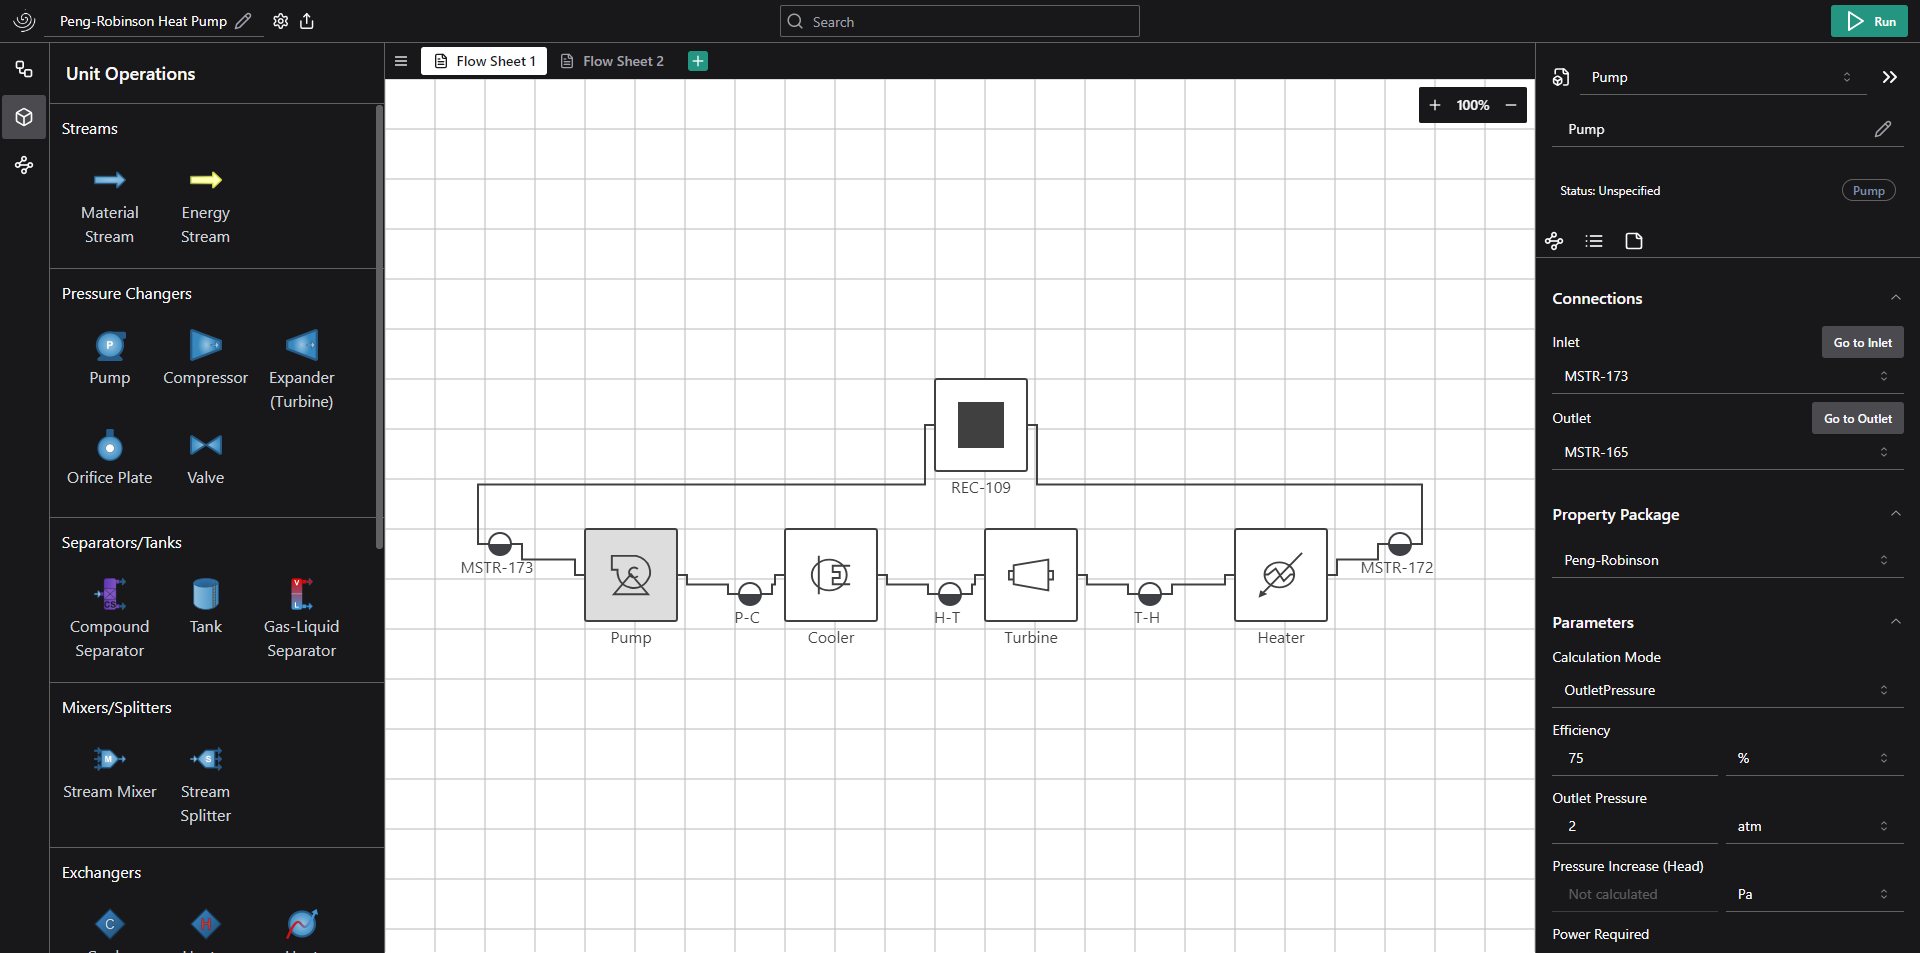
\includegraphics[width=\textwidth]{platform_screenshot.png}
    \caption{Example Flowsheet in the Ahuora Simulation Platform}
    \label{fig:platform}
\end{figure}

\Cref{fig:platform} shows a screenshot of the Ahuora Simulation Platform, as at August 2024. The user interface is divided into three main sections. The left-hand panel shows a list of unit operations from a factory, including pumps, heaters, heat exchangers, reactors, and material streams. The user can drag and drop these unit operations onto the canvas in the centre of the screen. The user can then connect the unit operations together to create a process flow diagram. The right-hand panel shows the properties of the selected unit operation, such as the flow rate of the material stream, the temperature and pressure of the stream, and the efficiency of the unit operation. The user can edit these properties to simulate different scenarios.

The displayed flowsheet shows a simple heat pump cycle. The block on the top is a ``recycle", specifying that the output of the cooler is fed back into the pump. A more complex flowsheet would replace the cooler and heater with heat exchangers, which exchange heat with their environment, but this provides a simple example.

\subsection{Online Integration}

\begin{figure}
    \centering
    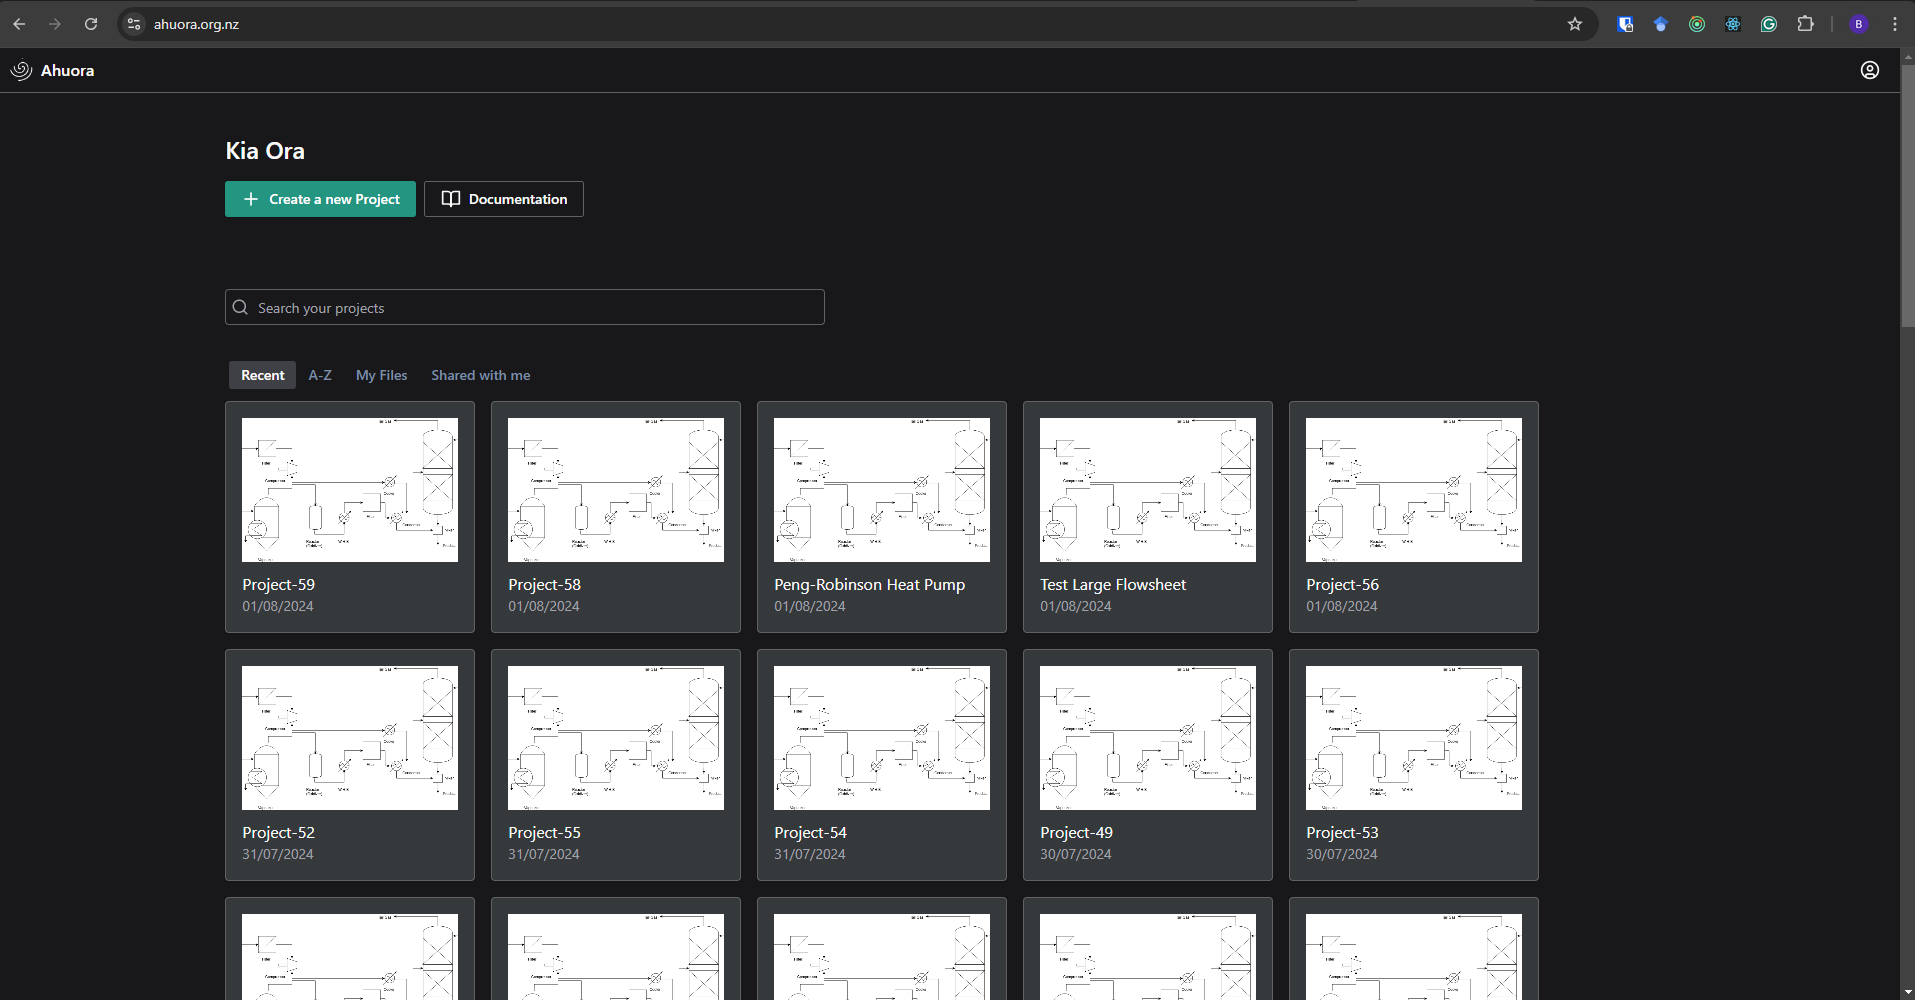
\includegraphics[width=\textwidth]{platform_homepage.png}
    \caption{Homepage of The Ahuora Simulation Platform}
    \label{fig:homepage}
\end{figure}

The Ahuora Simulation Platform is designed as a web-based multi-user platform. This offloads processing and data storage to the server, allowing users to access the platform from any device with a web browser. Simulation can be very computationally expensive, particuarly in advanced models, so this is a key feature. It enables simulation to be run in parallel on powerful servers, as the simulation is not done within the local web browser, but rather via distributed server infrastructure. This allows the platform to be used in industry without requiring significant upfront investment in hardware. 

In future, this will also enable the platform to be used for real-time collaboration between multiple users. Its API allows it to be integrated with other software, enabling enhanced functionality, real-time updates, and broader interactions.

The home page of the platform, shown in \Cref{fig:homepage}, provides a list of saved simulations, and allows the user to create a new simulation. This is not publicly acessible, as the platform is still in development, and user account functionality is not yet complete.

\section{Platform Architecture}

\begin{figure}[h]
    \centering
    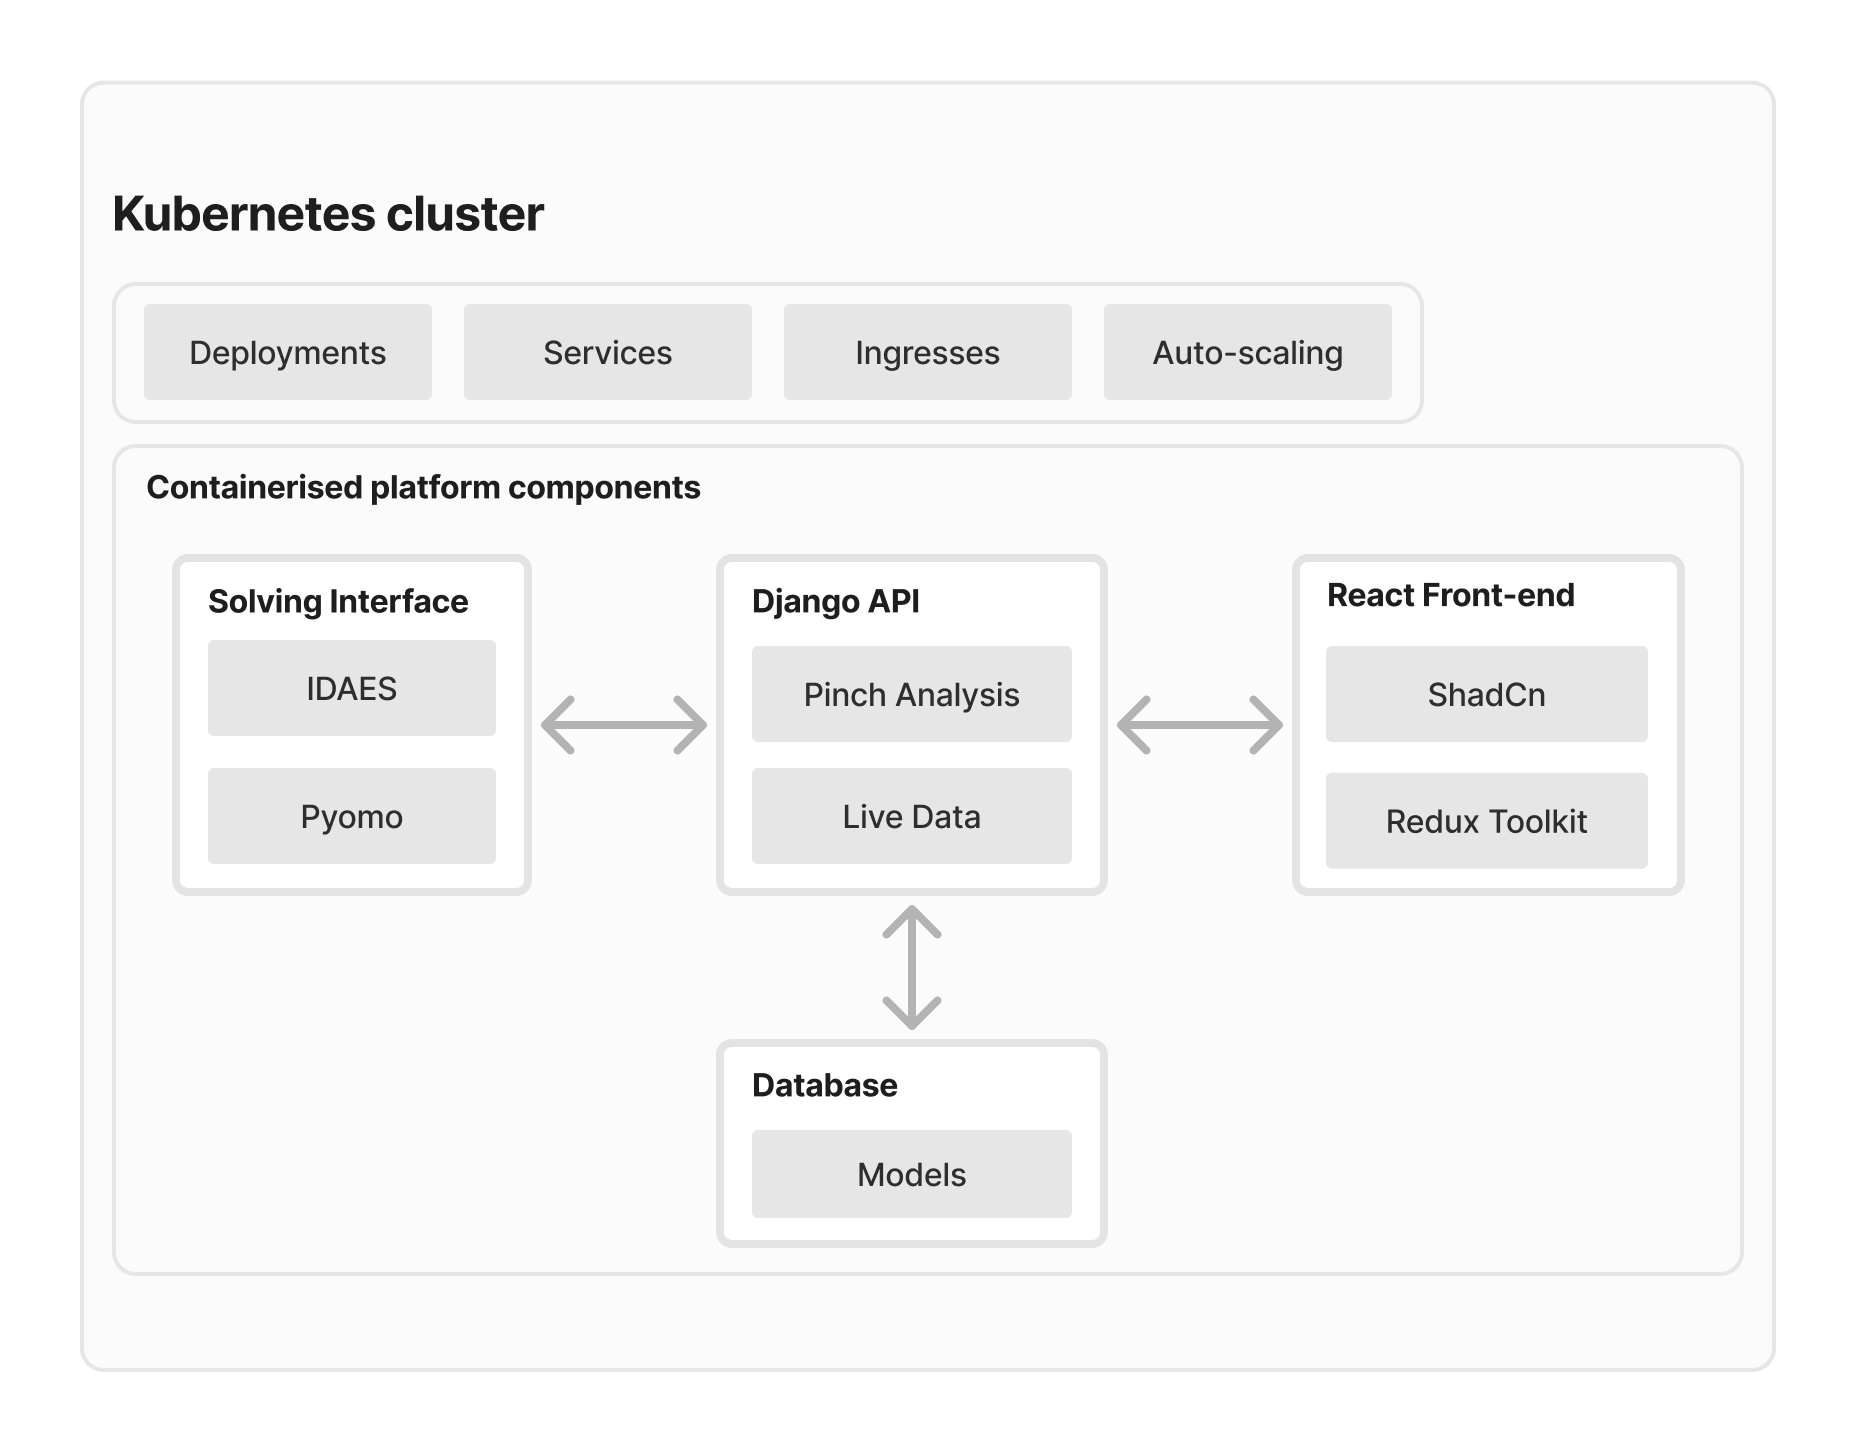
\includegraphics[width=\textwidth]{dt_arch.png}
    \caption{Architecture of the Ahuora Digital Twin Platform}
    \label{sec:platform_architecture}
\end{figure}

The platform is hosted in a Kubernetes cluster, located on-site. The Kubernetes cluster handles all web traffic, deployments from the private Github Repository, and scaling of services. 

Within the platform there are various containers running through the Docker platform, that can be replicated as required to scale based on service demand. The Database stores all flowsheets and model data. The solving interface uses the IDAES Process Simulation software~\cite{lee2021idaes}, built on the Pyomo equation-oriented modelling language~\cite{bynum2021pyomo}, to simulate a factory in real time. The User Interface is written in React Typescript, and uses the ShadCN UI Library and Redux Toolkit for state management and communication with the Django Backend. The Django API links all the services together, and handles the business logic for functionality such as Pinch Analysis and Live Data processing.

\section{Ongoing Projects}

Multiple other projects are being completed in parallel by other team members. Each project has a distinct topic, and is largely independent, but collaboration is required to ensure that each other's work is compatible.The projects cover a variety of topics, from analyis and data processing, to usability and deployment.

\subsection{Live Data Processing}

\textbf{Team Member Responsible:} Bert Downs

The Ahuora Platform currently supports building and simulating a factory, but it has no functionality to link live data from a factory into the Ahuora Platform. By integrating real-time sensor data into the simulation, the platform can monitor the factories' performance, and suggest tunings that will optimise resource efficiency. The data can also be used to predict and avoid failures and downtime, a key problem where many resources are wasted. Additionally, models created in the Ahuora Simulation Platform during the design phase could also be used during operation, minimising overhead costs.

\subsection{Pinch Analysis}

\textbf{Team member responsible:} Ethan MacLeod

One of the key optimisation tools the Ahuora Platform provides is the Pinch Analysis module. Pinch analysis is the process of identifying heat recovery pockets in a given system, and indicating where heat can be exchanged. The end goal of pinch analysis is reducing the overall heat consumption of a process, which in turn results in lower operational costs for a plant, and less greenhouse gas emissions produced. From the processes that are modelled on the Ahuora Digital Twin Platform, there is a distinct need for integration with process optimization tools like Pinch Analysis to inform the decision-making process for operators and engineers.

\subsection{User Interface Usability}

\textbf{Team member responsible:} Shean Danes Aton

This project aims to deliver an intuitive user interface and quality user experience in the Ahuora Digital Twin Platform through improving its UI through employing user centred methodologies including A/B testing, interviews, card sorting, the thinkAloud method, and surveys. Additionally, modern diagramming tools were reviewed and end users' knowledge were leveraged to the development of the ADTP UI. This project utilises software technologies and existing design components,ShadCn, for design implementations. Enhancing ADTP's UI increases user satisfaction, increases productivity, and minimises operational error.  

\subsection{Distributed Platform Deployment}

\textbf{Team member responsible:} Caleb Archer

Each of the software components making up the platform need to be deployed together within a distributed environment that allows for efficient allocation and use of computational resources. This is achieved within the context of a Kubernetes cluster, on which several replicas of each platform component may run at any given time based on system load. The ability to scale workloads in response to demand increases the capacity of the platform to perform process modelling and simulation, and handle a greater number of users.

\section{Other Long-term Platform Objectives}

The projects listed pave the way for future work on the Ahuora Digital Twin Platform. This includes expanding the number and type of unit operations supported, and supporting a wider range of chemical processes. It is intended that the Ahuora Platform also support Hybrid modelling, where Machine Learning Models are used to represent complex unit operations that do not have an exact mathematical representation. Analysis functionality to be added includes Dynamic Simulation, to model the factory over time and predict the effect of changes in the system, Process Variable Optimisation, to calculate optimal operating conditions, common diagramming and reporting functionality, and scheduling tools.

Because of the long-term context of the Ahuora project, work in this dissertation is constrained by the future requirements of the system. Care has been taken to ensure that the methods outlined can be extended to support the future objectives of the Ahuora Platform.

\chapter{Methodology}
% helicopter view, structure of the report

Software Engineering principles are notoriously hard to follow in academia \cite{connolly2023software}, partially because of of competing criteria for success. 
In academia, the criteria is publication of results, but in Software Engineering, creating and publishing a quality piece of software is quintessential to success. 
Additionally, since this project is conducted as part of a wider effort to improve the Ahuora Platform, research and development often had to account for a changing environment. 
Thus Agile principles were followed for both research and development, focusing on implementing one feature at a time. 

This project follows the ``Action Research'' methodology reviewed by Wohlin et al.~\cite{wohlin2021guiding}. The Action Research methodology is an iterative process, which includes five phases:

\begin{enumerate}
    \item Diagnosing - Identifying a problem to be addressed. The larger problem has already been identified in the Introduction and Literature Review. Each chapter also starts by identifying specific research questions, or the purpose of implementing a feature.
    \item Action Planning - Deciding what approach will best solve the problem. This is done by deciding on a prototype to build or a feature to implement, which is done at least once in each chapter.
    \item Action Taking - This involves setting the planned actions into practice - by building a prototype for research purposes, or implementing a feature in the Ahuora Platform.
    \item Evaluating - Studying and discussing the consequences of an action. The effectiveness of a prototype or feature, along with any other insights from the development process, is discussed at the conclusion of each chapter.
    \item Specifying/learning - Identifying general findings related to the problem under study. This is done explicitly in some chapters, such as by identifying the requirements of different types of users. The report is concluded with a chapter specifically devoted to generalising the findings of each previous chapter into a theoretical framework that can be used for implementing Digital Twins, and an implementation plan for the Ahuora Platform. 
\end{enumerate}


\section{Overview of Work}

\begin{table}[ht]
    \centering
    \caption{Overview of chapters}
    \label{tab:research_chapters}
    \begin{tabular}{|L{4.5cm}|p{11.5cm}|}
    \hline
    \textbf{Chapter} & \textbf{Purpose} \\
    \hline
    Data Collection \mbox{(\Cref{sec:heatpumpcollection})}& Understand the process of collecting data from a thermodynamic system, using a Heat Pump Dryer as a test case. \\ \hline
    Simulation Technologies \mbox{(\Cref{sec:architectureresearch})}& Identify potential analysis techniques for a Digital Twin system, and what is required to make use of them. \\\hline
    Prototyping \mbox{(\Cref{sec:simulationprototype})}& Experiment with linking live data to a simple simulation in the Ahuora Platform. \\\hline
    Recording History \mbox{(\Cref{sec:history})}& Adding the ability to store past solves in the Ahuora Digital Twin Platform. \\\hline
    Data Preprocessing \mbox{(\Cref{sec:datapreprocessing})}& Functionality for parameterising solves, to make it easier to develop Digital Twins. \\
    \hline
    \end{tabular}
\end{table}

Each chapter has a distinct objective, yet each piece of work contributes to the same high-level objectives. \Cref{tab:research_chapters} summarises the specific focus of each chapter. 
Chapters \ref{sec:heatpumpcollection} \& \ref{sec:architectureresearch} focus on understanding the core tools and platforms that relate to Digital Twin solutions, establishing a holistic long-term view of the problem. These chapters are more research focused.

Chapter \ref{sec:simulationprototype} assesses the conclusions from the previous chapters, by building a prototype live data collection system. A theoretical framework is presented that can be used generally to inform Digital Twin development efforts. 

Chapter \ref{sec:history} develop some features in the Ahuora Simulation Platform that implement characteristics discussed in the earlier chapters. The features discussed in this section are now integrated into the Ahuora Platform codebase.

A case study of a heat pump dryer was used throughout the report to evaluate the prototypes built and features developed.  This was achieved by developing a model of a heat pump dryer in the Ahuora Simulation Platform, and integrating real-time sensor data into the model. The case study was used to evaluate the feasibility of the framework, and to identify areas for future work.

\part{Research}
\chapter{Data Collection: The Heat Pump Dryer} \label{sec:heatpumpcollection}

\section{Purpose}

The literature review identified that the inputs to the Digital Twin Platform would be sensor data from the lower-level data collection software, and the outputs would be results from  the simulations performed by the platform. To be able to test our processes, input data was required, so a Heat Pump Dryer was chosen.

A Heat Pump Dryer provides a good test case for live data processing. Heat Pumps are a common unit operation in chemical plants. A heat pump models most thermodynamic operations, including heat exchangers, compressors, and expansion valves, including the effects of phase changes. The inclusion of a refrigerant loop makes it a good test case as recycle processes are common in industry. Gathering data from the heat pump dryer will provide some insights into the challenges involved in real-time data collection.

Since the Heat Pump Dryer includes its own control system, it does not provide a test case for closed-loop control. This is out of scope and will be a future area of research.

\begin{figure}
    \centering
    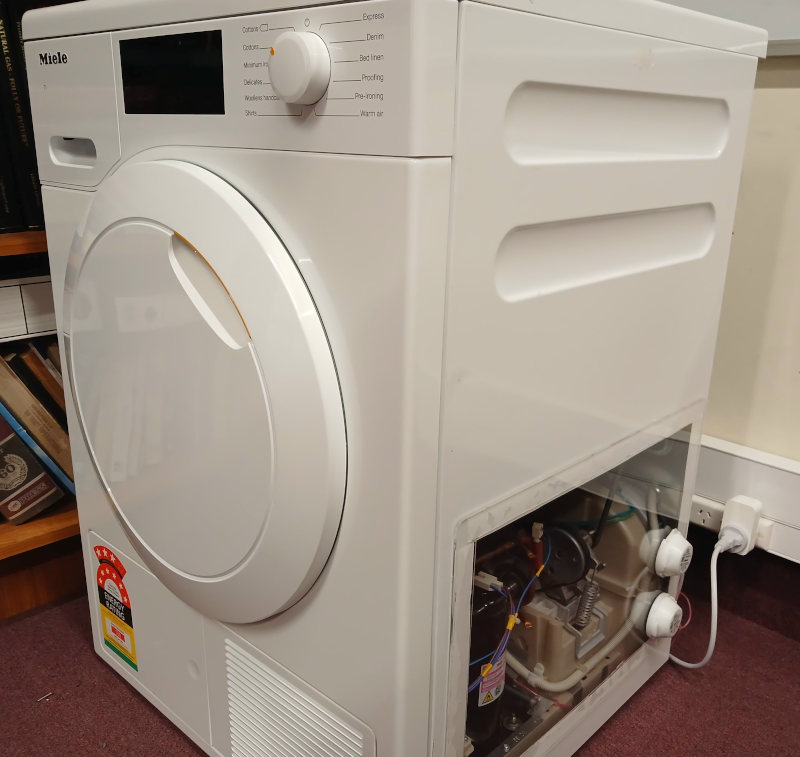
\includegraphics[width=0.4\textwidth]{dryer.png}
    \caption{Heat Pump Dryer}
    \label{fig:dryer}
\end{figure}

\section{Method}


To gather data from the heat pump dryer, Bluetooth sensors were used to measure temperature and humidity at various points in the dryer. A power meter was used to measure the total power consumption of the heat pump dryer. A raspberry pi was used to collect the data from the sensors, and store it in a InfluxDB time-series database. InfluxDB was chosen because it is one of the platforms identified in the Literature Review as being used for aggregating sensor data; it is also open-source and easy to use. This can represent the data collection system that would be used in industry.


\begin{figure}
    \centering
    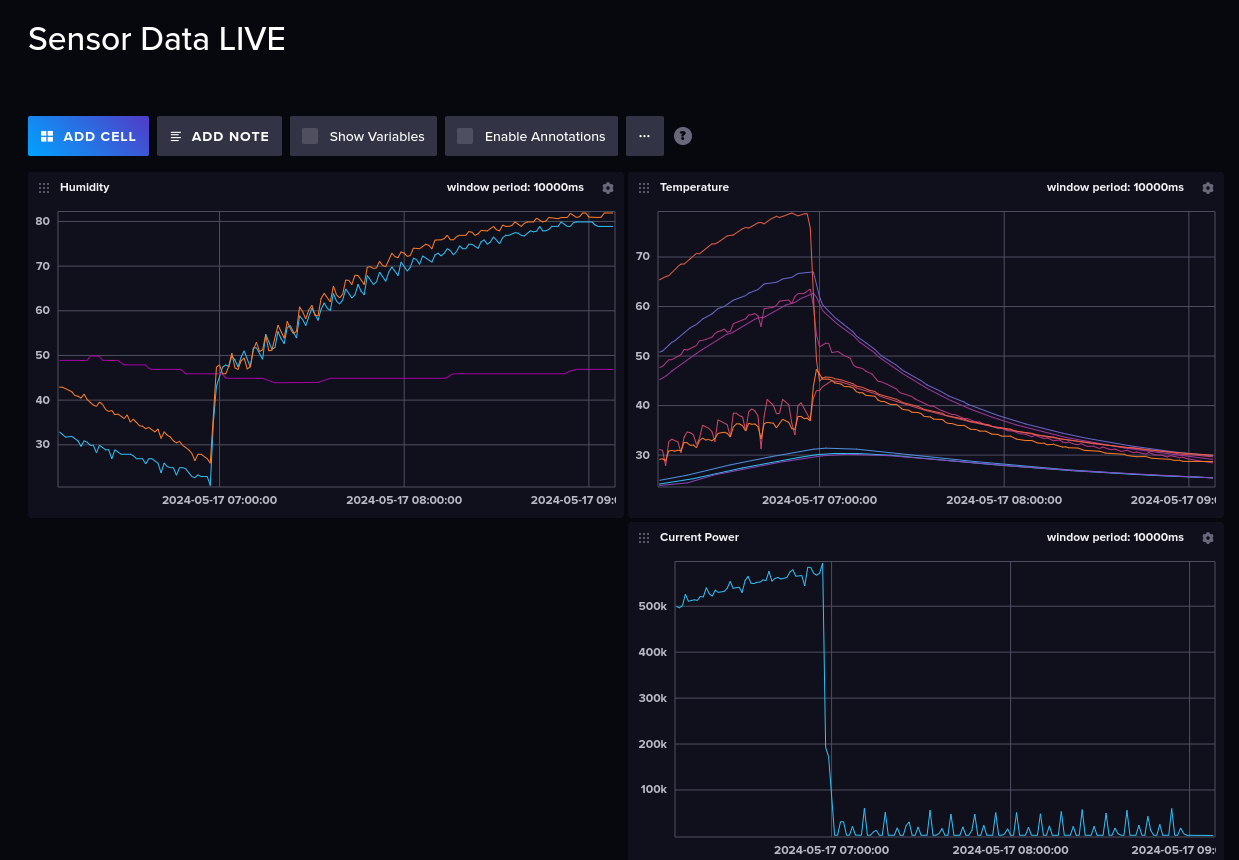
\includegraphics[width=\textwidth]{influxdb.png}
    \caption{InfluxDB Database}
    \label{fig:influxdb}
\end{figure}

\section{Insights}

The process of gathering and aggregating data was relatively straightforward. This reinforces the finding from the literature review that there are a number of tools already available for collecting and processing sensor data. 

Depending on the process, there is often only a limited amount of information that can be gleaned from the system. For example, we were not able to collect pressure information, as pressure sensors are more costly and require modification of the refrigerant loop. Likewise, we were only able to measure the total power consumption of the heat pump dryer, rather than the power consumption of individual components. Data processing techniques will need to be able to infer the state of the system from the limited data available.

Additionally, in operation, the heat pump dryer has a number of different operating cycles: it does not just continuously run all of the time: sometimes it switches direction, etc. This changes the state of the system, so the simulation will need to be able to account for this. We did not have access to the control system of the heat pump dryer, so we were unable to collect data on the operating cycles. Depending on the setup in industry, this data may or may not be avaliable.


\chapter{Architecture Research} \label{sec:architectureresearch}

The literature review also identified a variety of modelling techniques, including Steady-state modelling, Dynamic Modelling, Surrogate Modelling, and Optimisation. 

The Ahuora Digital Twin Platform is currently built to support only steady state modelling. However, to explore the potential for integrating more advanced live data processing techniques, the IDAES Process Systems Engineering Framework was employed as a testbed.

The IDAES framework is a Python library that provides tools for modelling and simulating chemical processes. It is designed to be extensible, allowing for the addition of new modelling techniques.

Using the IDAES framework, experimentation with live data processing techniques was undertaken. This testing aimed to evaluate the feasibility of integrating these advanced techniques into the Ahuora Digital Twin Platform. By leveraging IDAES, the platform can be designed to support the incorporation of more sophisticated modelling techniques in the future.

\section{Research Questions}

The research investigation aimed to answer the following questions:

\begin{itemize}
    \item \textit{RQ1:} How does the Ahuora Simulation Platform need to be modified to support dynamic modelling, surrogate modelling, and optimisation?
    \item \textit{RQ2:} What architecture would best support the integration of live data processing techniques into the Ahuora Digital Twin Platform?
\end{itemize}

\textit{RQ1} focuses on future needs and long-term vision. This is important to help minimise the amount of rework required when implementing new features. \textit{RQ2} focuses on the immediate needs of the project, and is important for developing a pilot implementation.

\section{Dynamic Modelling} 

The IDAES framework was used to develop a dynamic model of a steam tank, with a valve controlling the inlet and outlet pressure and flow rate. A PID controller was used to control the valve opening fraction to regulate the pressure in the tank.

\begin{figure}
    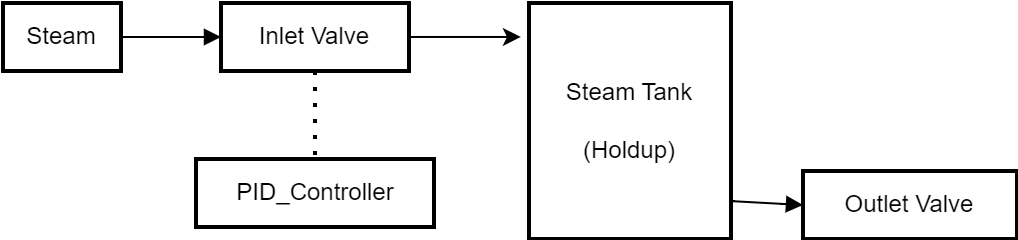
\includegraphics[width=0.9\textwidth]{dynamicmodelling.png}
    \caption{Dynamic Modelling of a Steam Tank}
    \label{fig:dynamicmodelling}
\end{figure}

This provided a simple example of a dynamic system. The inlet and outlet valve and the PID controller were not dynamic models: From a mathematical perspective, this means their properties were fully determined by the inlet and outlet conditions. The only dynamic model was the Steam Tank. From a mathematical perspective, this means that the state of the steam tank was determined not only by the the inlet and outlet conditions, but also by the previous state of the tank, i.e how ``full" the tank is.


\section{Analysis}\label{sec:dynamicmodelling}

\begin{itemize}
    \item The IDAES framework is well-suited to dynamic modelling, as it provides tools for creating and solving differential equations. It can easily model the same system at different time scales.
    \item The Ahuora Simulation Platform requires substantial changes to support dynamic modelling. Rather than storing a single value for each property, it will need to store the state of each property at each time step.
    \item This also necessitates significant UI changes to view the state of the system at different time steps. This could be achieved through some sort of time slider, and graph visualisations of properties over time.
    \item Specifying the initial conditions of the system is more complex, as the user needs to specify the initial state of dynamic properties, such as the initial tank level. Other properties, such as the valve opening fraction, need to be specified as functions of time.
\end{itemize}

\section{Surrogate Modelling}
Surrogate Modelling is the process of creating a simplified model of a complex system. This is usually done using machine learning techniques. This provides a good test case for implementing data-driven modelling techniques within the IDAES framework.

IDAES includes a framework for data-driven modelling called PySMO. This provides utilities for training polynomial, Radial Basis Function (RBF), and Kriging models to approximate the behaviour of a system.

To test the workflow for hybrid modelling, a simple surrogate model is created using PySMO. First, a set of data points is generated by solving a heater model at different pressures, temperatures, and flow rates. 
Then, this data is used to train a surrogate model, which can predict the outlet pressure and enthalpy from the valve based on the inlet conditions. 
This generated data for a steady-state simulation, predicting the outlet pressures and temperatures. 
An RBF network is trained to predict these values from the inlet conditions.
The weights of the trained model are then saved to disk. 

\begin{lstlisting}[language=Python,caption=Using a surrogate model in IDAES,label=lst:heater_surrogate]
model = PysmoSurrogate.load_from_file('pysmo_heater_surrogate.json')
inputs = [self.inlet.pressure, self.inlet.temperature, self.heat_duty, self.inlet.flow_mol ]
outputs = [self.outlet.pressure,self.outlet.temperature,self.outlet_vapor]
self.surrogate = SurrogateBlock(concrete=True)
self.surrogate.build_model(model,input_vars=inputs, output_vars=outputs)
\end{lstlisting}

To use the surrogate model in a flowsheet, the weights of the model are loaded and the structure of the model is recreated as a set of algebraic constraints, relating the input conditions to the predicted output conditions. This can be combined with IDAES's UnitModel class and StateBlocks to create a new unit operation that can be used in a flowsheet.

As shown in Listing \ref{lst:heater_surrogate}, each input and output is linked to a parameter in the unit operation. This works for steady-state models, but dynamic models have a set of parameters, so the surrogate model would need to be able to predict the next time step from the previous time step. This is a much more complex problem, as it would have to be time scale invariant.

\subsection{Analysis}\label{sec:surrogatemodelling}

Surrogate Modelling can be achieved using IDAES's built-in PySMO libraries, or other similar libraries such as OMLT. It is reasonably straightforward to train a surrogate model to represent a non-dynamic unit operation, but dynamic unit operations get significantly more complex - instead of modelling a single value, the surrogate model must be able to model the entire time system. There are some methods of doing this, such as using neural ODEs, Residual Networks, Operator Networks, or some other sort of convolutional network. There is little research into applying these methods in the field of chemical and process simulation, especially in the context of mathematical modelling such as the IDAES framework.

The exact same process for surrogate modelling can also be used to model unit operations from historical data. This is useful when there is no mathematical model of the unit operation, but there is historical data available. This is very useful when considering the application of the Ahuora Digital Twin Platform to existing factories, where the exact mathematical properties of the unit operations are unknown but there is a wealth of historical data available. Online Learning techniques could be used to update the surrogate model in real-time, as new data becomes available. This is a key step in turning a ``simulation" into a ``digital twin", as it allows the model actively adapt to real-world conditions.

Because of the limited functionality of the Ahuora Digital Twin Platform, it is currently beyond the scope of this project to implement a surrogate model. However, the IDAES framework is well-suited to this task, and it is likely that a surrogate model could be implemented in the future.

Additionally, the Ahuora Digital Twin Platform will need a user interface to support creating these different types of models. As surrogate modelling is a complex process, the user interface will need to be able to guide the user through the process of creating a surrogate model from a dataset, and provide feedback on the quality of the model. This will require a significant amount of work, and will likely be a key focus of future development.


\section{Optimisation and Control}

Optimising a system involves adding an objective the model using standard Pyomo utilities, and then solving the model to find the optimal conditions. In the heater model, a cost function is added as a test objective, to find the ideal balance between heat duty and outlet temperature. The model is then solved to find the optimal heat duty that minimises the cost function.

\begin{lstlisting}[language=Python,caption=Optimising the heater model in IDAES,label=lst:optimisation]
def cost_objective(h):
return 3**(h.heat_duty[0]/5000) - (h.outlet.temperature[0]-350) * 33000
m.fs.heater.cost_objective = pyo.Objective(rule=cost_objective, 
                                           sense=pyo.minimize)
\end{lstlisting}

This is shown in Listing \ref{lst:optimisation}. The model must be solved with degrees of freedom, i.e variables that the solver can adjust to find the optimal solution. In this case, the heat duty is the degree of freedom, but there can be multiple degrees of freedom in a model. 
In \Cref{fig:optimisation_dynamics}, a setpoint function for the outlet temperature is added, and optimisation is used to find the heat duty for each timestep such that the resulting outlet temperature best tracks to the setpoint. This has one degree of freedom for each discrete time step that must be optimised: the heat duty at that time step. 
When this technique is used to control a system based on the optimal way to reach a setpoint, it is referred to as Model Predictive Control.
Because the setpoint change is instantaneous, it is unable to perfectly follow the setpoint, but is able to minimise the error on either side of the setpoint through controlling actions. 

\begin{figure}[h]
    \centering
    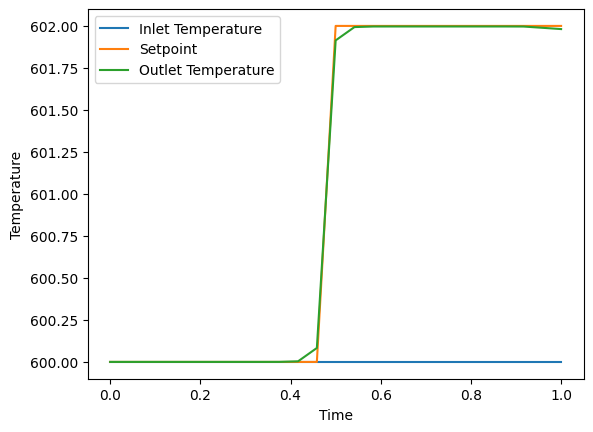
\includegraphics[width=0.6\textwidth]{research_article/dynamics_optimisation.png}
    \caption{Optimising a dynamic model to follow a setpoint.}
    \label{fig:optimisation_dynamics}
\end{figure}

The optimisation technique used here could be used iteratively for model predictive control, where the model is solved at each time step to find the optimal control action. 


\subsection{Analysis} \label{sec:optimisationcontrol}

Implementing Model Predictive Control in IDAES is relatively straightforward, as long as there is a dynamic model of the system, a cost function, and the optimisation problem is well-posed. The Ahuora Digital Twin Platform does not support optimisation yet, but this will be supported in the future.

In order for model predictive control to be useful, IDAES needs to be paired with a real-time data processing system. The real-time data processing system will need to be able to actuate the suggestions of the MPC simulation in real-time, and then inform the MPC simulation of the system's response. This requires integration with the industry-specific SCADA systems that are used to control factories.

\section{Theoretical Architecture} 

Conventional simulation platforms do not have built-in support for live data processing. Likewise, conventional factory SCADA\footnote{SCADA systems: Supervisory Data Aquisition and Control systems.} systems do not have built-in support for complex simulation. To integrate a simulation platform with live data, a software system must be created that can merge the two systems. This can be considered as an intermediate layer between the simulation platform and the factory SCADA system.


\begin{figure}[h]
    \centering
    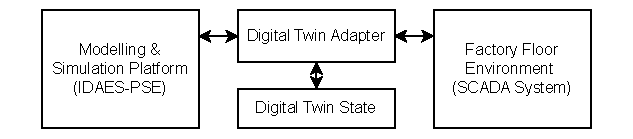
\includegraphics[width=0.8\textwidth]{research_article/research_journal_framework_simple.pdf}
    \caption{Theoretical framework of how a Digital Twin can be implementend on top of existing simulators and factory control systems.}
    \label{fig:theoretical_framework}
\end{figure}

The concept of a “Digital Twin” refers to a simulation of something in the physical world, which is kept up to date with a physical system using real-time data \cite{yu2022energy}.
In \Cref{fig:theoretical_framework}, this intermediate layer is what converts the simulation platform, and the data from the factory, into a digital twin. 

By breaking the Digital Twin up into these core components, we are able to make use of existing software systems for live data processing and simulation, and only need to build the components that are unique to the Digital Twin use case. This limits the complexity of the system, and means that implementing a Digital Twin in a factory can be done with minimal disruption to the existing systems.

% These sections should be presenting the arguments that we will make in all the other sections.

\subsection{Modelling and Simulation Platform}


Being able to model and simulate a process is one of the foundational components of a Digital Twin platform. 

Conventionally, simulation platforms are used when designing and planning a factory, and are not used during operation. This makes most conventional simulation platforms unsuitable for use in a Digital Twin, without substantial modification.
In the Ahuora Platform, IDAES-PSE provides the core modelling and simulation capabilities. 
It is built on top of Pyomo, an Algebraic Modelling Language, enabling for flexible model definitions.
This flexibility is key in enabling a Digital Twin platform to be built on top of IDAES. 
Further flexibility is enabled through the Ahuora Platform, which can be modified to support whatever features are required.

% Todo: Give Examples, link to sections that go through the different parts
\subsection{Factory Floor Environment}

In the factory, there are many sensors and control systems that monitor the state of the factory. These systems are often connected to a SCADA system, which is responsible for collecting and displaying this data.
Additionally, there are often data processing systems that are used to store and process this data, as historical data is often used in later analysis to improve performance or make maintenance and upgrade decisions.

There are also automated and manual control systems, which are used to adjust the factory's operation based on the data collected by the SCADA system.
These systems are already implemented in factories, and are critical to the operation of the factory.

% Todo: Give Examples, link to other sections
\subsection{Digital Twin Adapter}

As such, rather than making a new data processing system, it is better that a Digital Twin Platform can be built such that it can be implemented on top of established data processing systems. Likewise, rather than making a new simulation platform, it is better if the framework of an existing simulation platform can be reused or adapted to the digital twin use case.

The concept of a ``Digital Twin Adapter'' is used to define this functionality. It is responsible for converting the data from the factory into a format that the simulation platform can understand, and to provide results from simulations back the factory.


% Todo: give examples, link to other sections
\subsection{Digital Twin State}

Key to the sucessful operation of the the Digital Twin Adapter is the fact that is also has access to the ``Digital Twin State". The Digital Twin State represents an estimate of the current state of the factory, based on the simulation results and the live data. 
This represents the ability of a Digital Twin to "learn" how the physical system behaves, and adjust the inputs to the simulation accordingly.



\section{Discussion} \label{sec:researchconclusions}

The architecture presented generalises the concept of a Digital Twin, enabling software to be built that can be used in a wider variety of factories. However, the exact implementation of the Digital Twin Adapter may need to change depending on the factory's existing systems. Different SCADA systems and data processing systems will have different ways of communicating, and different data will be avaliable depending of the factory. Likewise, different methods of simulation may or may not be avaliable depending on the system. 

The Digital Twin Adapter will need to be built in a way that it can be customised or set up differently depending on the factory. 
% TODO: maybe the research conclusions should be seperated out, or put into the proposed architecture section.
% It makes more sense for the conclusions of this chapter to be about how each of the modelling techniques fit in to the proposed architecture, to argue that my architecture is correct.


The current Ahuora Simulation Platform is split into three main parts:

\begin{itemize}
    \item The Frontend UI, which is written in Typescript/React and runs in the user's web browser. This is responsible for rendering the flowsheet, and allowing the user to interact with the simulation.
    \item The Backend API, which is written in Python/Django and runs on the server. This is responsible for storing the simulation data, orchestrating calls to run the simulation, and returning the results to the user.
    \item The IDAES solving engine, which is written in Python and runs on the server. This is responsible for solving the simulation, and returning the results to the API. It has been seperated out from the API to allow it to be scaled independently.
\end{itemize}

Over time, the Ahuora Simulation platform will be expanded to support dynamic modelling, surrogate modelling, and optimisation.

Additionally, there are also a number of other tools that are used in industry for collecting and processing sensor data. There may be an integrated solution or a number of different tools that are used together, but they can be grouped by their functionality:
\begin{itemize}
    \item Data Collection: These tools are responsible for collecting data from sensors and storing it in a database, as well as cleaning and preprocessing the data. This includes IoT networks and SCADA systems.
    \item Data Processing: These tools are responsible for processing the data to extract useful information. This includes machine learning models, statistical analysis, or other data processing techniques. Generally, these tools will sit within some sort of framework or pipeline, such as Apache Kafka, Flink, or a custom solution.
    \item Data Storage: These tools are responsible for storing the data in a way that is accessible to the other tools. This includes databases, data lakes, or other storage solutions. In Model-Based Systems Engineering, this is often referred to as a Knowledge Base.
\end{itemize}

\begin{figure}
    \centering
    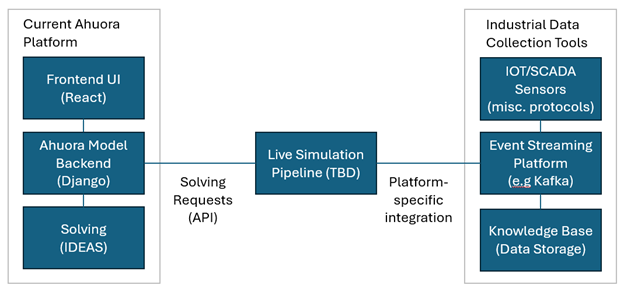
\includegraphics[width=0.9\textwidth]{architecture.png}
    \caption{Anticipated method of implementing the Ahuora Simulation Platform into an industrial system.}
    \label{fig:architecture}
\end{figure}

 Thus, a future requirement of the Ahuora Simulation platform is the connection to these tools to access the sensor data. However, there is a discrepancy in the use cases of the Ahuora Simulation Platform and the standard industrial stack. The Ahuora Simulation Platform is designed with experimentation and analysis in mind, which are usually offline\footnote{Many use cases of the Ahuora Simulation platform include designing new factories or modifications to a factory. These tasks mostly use historical data, and are a distinctly seperate problem from live prediction and control.} tasks performed by expert engineers. The standard industrial stack is designed for real-time prediction and control, which are online tasks performed by operators. Both the engineer and operator workflows will require all the modelling and simulation techniques identified, but the operator's workflow uses a fixed set of models.

\begin{table}[ht]
    \centering
    \caption{Comparison of Engineer's and Operator's Requirements}
    \begin{tabular}{|c|p{0.35\textwidth}|p{0.4\textwidth}|}
        \hline
        \textbf{Requirement} & \textbf{Engineer} & \textbf{Operator} \\
        \hline
        Use Case & Design, Retrofit, & Maintenance, Monitoring, Control \\
        \hline
        Modelling & Creates and modifies multiple models & Fixed set of models, only certain parameters may change\\
        \hline
        Data Usage & Historical data, likely preprocessed or cleaned & Real-time raw data \\
        \hline
        Reliability & It is acceptable if incorrectly configured models don't solve & Model must be correct; Requires 100\% reliability \\
        \hline
    \end{tabular}
    \label{tab:requirements}
\end{table}

Because of the different use cases, while the Ahuora Simulation platform needs to be designed so that it is easy to design and build a model, this functionality is not required in operation. The model could be considered ``frozen'' at this point, where only certain parameters can be changed based on the real-time data. It does not make sense to expose functionality to edit the model to an operator. 



Deploying the a model in production would likely only be done by a trained engineer who manages the plants' SCADA systems.
The deployment would have to be custom for each plant, depending on the SCADA system in use, the sensors available, and the model being used. 
Making a User Interface for this process would be very challenging, and would limit support to only a certain number of protocols. 
Thus, it can be considered that the interface, pipeline, or service between the Ahuora Simulation Platform and the SCADA system is a custom software component. 



%\chapter{Results: Recommended System Architecture} \label{sec:proposed_architecture}

% I'm thinking this could be a bit like a whitepaper, where I outline the requirements for the Ahuora Digital Twin Platform, and how I think it should be implemented.
% then the other sections can go into more depth, to confirm my argument that this is the best way to implement the platform.

% Digital Twin Software needs to suit the use cases of Network Administrators, Chemical Engineers, Process Engineers, and Operators to be useful in industry.
% Steady-State, Dynamic, and Surrogate modelling are all required to support the different use cases.
% A Digital Twin platform needs to integrate with existing SCADA systems and data processing tools to be useful in industry.

% Simulation results need to be avalible within the platform, but this should not replace the company's existing knowledge base/data lake/logging.
% There is no need for Ahuora to develop a new data processing platform, as SCADA systems or things such as kafka/mqtt do this fine.
% It should be easy to switch between design and operation modes, assuming the network administrator has set up the external data processing platform/sources.
% The Ahuora Digital Twin Platform needs to be designed to support these requirements.

% What Hypothesis am I testing here?
% How do I recommend that the above be implemented?


% Todo: Give examples, link to other sections.




\chapter{Prototype: Live Data Simulation} \label{sec:simulationprototype}

\section{Purpose}

The purpose of the prototype was to demonstrate how the Ahuora Simulation Platform could be integrated with a real-time data processing system. It was designed to be a minimum-viable product, demonstrating the feasibility of the architecture developed in the research stage. As appropriate, it could form the basis of a more comprehensive framework, or provide insights into the requirements of a future system.

\section{Method}

\begin{wrapfigure}{r}{0.5\textwidth}
    \centering
    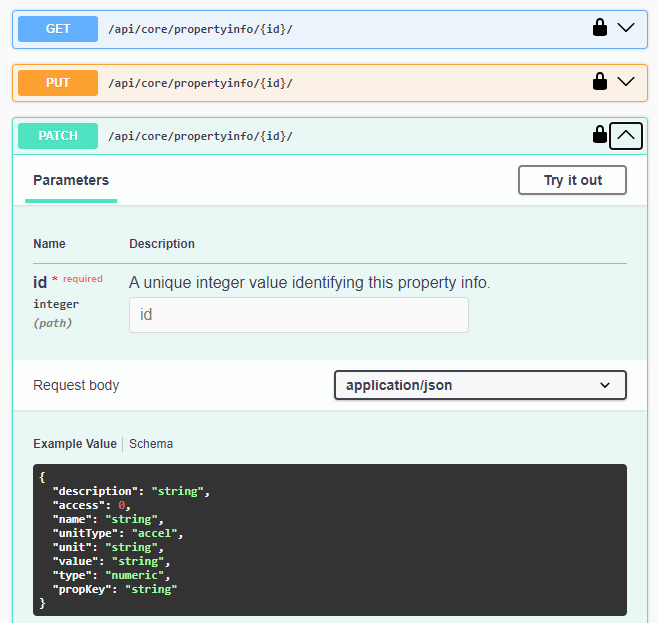
\includegraphics[width=0.5\textwidth]{swaggerprops.png}
    \caption{Swagger definition of API endpoints for updating properties.}
    \label{fig:swaggerendpoints}
\end{wrapfigure}

The Ahuora Simulation Platform has a REST API that is used internally to communicate between the frontend and the backend. This API already includes endpoints for updating properties, and retrieving properties after a simulation. This api could also be used for real-time data processing systems to communicate programmatically with the platform.

Each property field has a unique ID, generated by the database. The flowsheet needs to be set up ahead of time with the relevant unit operations, and properties. To solve the flowsheet repeatedly based on real-time data, the properties in the flowsheet can be updated to reflect the real-time state programmatically, and then a call can be made to the API endpoint to solve the flowsheet. Then, relevant properties can be queried to get the results of the simulation.

\begin{figure}
    \centering
    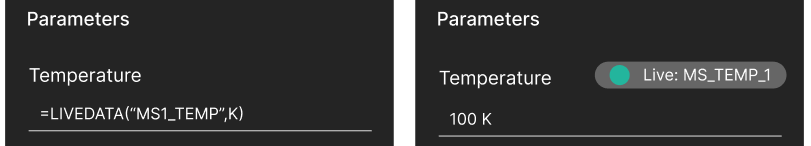
\includegraphics[width=0.8\textwidth]{property_ui.png}
    \caption{Prototype UI designs for setting a property as a ``real-time'' property.}
    \label{fig:property-ui}
\end{figure}

As the property IDs are generated by the database, it does not make sense to hard-code them into the real-time data processing system. There should be a more generic way of referring to properties that need to be updated. Some prototyping of a UI method to set properties as ``real-time'' in the existing interface was done, as shown in \cref{fig:property-ui}. This would allow the user to select which properties should be updated in real-time, and provide a way to refer to them in the real-time data processing system. However, ultimately we decided not to implement this yet, partially because it did not provide a clear separation between the engineers workflow and the operators workflow, and partially because it was not necessary for the prototype.

Instead, we used a simple definitions file to map the properties in the Ahuora Simulation Platform to the properties in the real-time data processing system. As shown in \cref{fig:live-constants}, the file included the unit operation name, the property key (used by the Ahuora Simulation Platform to determine property types), and the sensor ID from the real-time data processing system. The data processing platform could use this information to find the property IDs in the Ahuora Simulation Platform, and update them with the real-time data.

\begin{figure}
    \centering
    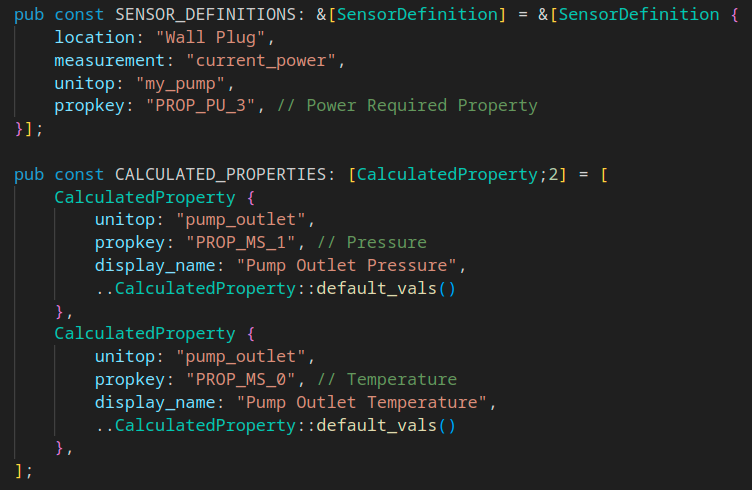
\includegraphics[width=0.8\textwidth]{live_constants.png}
    \caption{Definitions file for mapping properties in the Ahuora Simulation Platform to the real-time data processing system.}
    \label{fig:live-constants}
\end{figure}

Rather than truly connecting it to real-time data, for now the prototype used a CSV file with dummy data in the same format as the real-time data collected in \cref{sec:heatpumpcollection}. This was simply to make debugging and testing easier; the process would have been the same if the data was being read from the sensors live.

This prototype also used a very simple model: a pump with an inlet stream and an outlet stream. The power used by the pump was calculated based on the  ``live'' data, and the inlet streams were already specified. The simulation would be used to calculate the outlet pressure and temperature of the pump. This was a simple model, but it was sufficient to demonstrate the feasibility of the architecture.

% TODO: Add image: Running the simulation on the CSV file.

When the script was run, for each new data point, the script would update the properties in the Ahuora Simulation Platform, and then call the API to solve the simulation. The results of the simulation were then printed to the console. 

This worked suprisingly well, and was able to be done in only around 300 lines of code. It was implemented in Rust, using an API client SDK generated from the OpenAPI specification of the Ahuora Simulation Platform. This made it fully type-safe and reliable. Because of the configuration file format, it would be trivial to add a longer list of sensors and calculated properties, as would be required in more complex properties.

\section{Insights} \label{sec:prototypeinsights}

This prototype significantly affected the focus of future work. The prototype demonstrated that the Ahuora Simulation Platform could be integrated with a real-time data processing system with relatively little effort, as long as there was a standardised API. Sure, depending on the type and quality of the sensor data, there may need to be some data cleaning and preprocessing, but that is use-case specific business logic. Hence, there may be little need to develop a standardised data preprocessing pipeline or service for the Ahuora Digital Twin Platform.
To confirm this, the heat pump dryer will be used as a case study in linking a more complex system (with custom business logic required) to the Ahuora Simulation Platform.

This approach, which closely follows the architecture described in \cref{fig:architecture} in \cref{sec:researchconclusions}, also outsources the processing, visualisation, and control actions to third-party systems, as all data would be stored in the factory's existing knowledge base after processing, completely external to all Ahuora Systems. In some ways, this is a good approach: it could be easy to make a "headless" version of the Ahuora Simulation platform that can be deployed with a single frozen model, into a factory's existing systems. This would be good for stability and reliability reasons, limiting the complexity of the system. This is the unix ``do one thing and do it well" philosophy applied to software architecture.

However, there are disadvantages to this approach. One of the key value propositions of the Ahuora Digital Twin Platform is that it provides one place to define a factory's architecture, and then multiple types of analysis can be used on it. The same structures could be helpful for automatically creating visualisations of the real-time state of the factory, fault diagnostics, control, and surrogate modelling. As the platform currently stands, it cannot be considered a ``Digital Twin'', true digital twins include multiple fidelities of simulation, and dynamic ``state'' that adapts to real-world conditions via a feedback loop. The next steps in development will need to balance these two approaches, to find an architecture that includes the advantages of each.

%\chapter*{\textit{Interlude: Transitioning to Development}} \label{sec:interlude}
\addcontentsline{toc}{chapter}{Interlude: Transitioning to Development}

% TODO: Review this section

Up until this point, the project has been focused on experimentation, research, and prototyping. Chapters \ref{sec:heatpumpcollection} through \ref{sec:simulationprototype} have identified key use cases, requirements, and architectures for processing live data. 
\Cref{sec:heatpumpcollection} identified that while data collection is straightforward, there are limitations to the data that can be collected. Often, custom logic for inference or sensor fusion will be required. \Cref{sec:architectureresearch} tested the conclusions from the literature review, concluding that IDAES is capable of supporting dynamic modelling, surrogate modelling, optimisation, and control, but that these features mean different things in the context of live data processing compared to offline simulation. \Cref{sec:simulationprototype} demonstrated that the Ahuora Simulation Platform could be integrated with a real-time data processing system for steady-state modelling with relatively little effort, as long as there was a standardised API, and provided techniques to do so. However, much more complexity arises when combining all these concepts together, and when balancing the needs of the engineer's workflow with the operator's workflow.

The best way to prove the efficacy of this system is to start building it. Even though the perfect architecture has not yet been found, it is quicker to build a system and iterate on it than to try to design the perfect system from the start. The following chapters are focused on developing the Ahuora Simulation Platform to support live data processing, and iteratively testing these developments on the Heat Pump Dryer Model.

The research conducted so far has provided the context required to build a high-level roadmap of future development. This is shown in \cref{fig:development_flowchart}, where the development is broken down into phases. Each phase is broken down into subtasks, identifiying the key challenges to overcome.
Phase 1 provides the core functionality: ingesting data, solving the simulation, and displaying the results. This is the minimum viable product, and constitutes the main objective of this project. Phase 2 adds support for physics based modelling, optimisation, and control. The key challenges anticipated, including specifying input of the the time domain, holdup, and visualisation, come from the research conducted in \cref{sec:dynamicmodelling}. Likewise, the key challenges from optimisation and control originate from the research in \cref{sec:optimisationcontrol}. Based on research from the literature review and \cref{sec:surrogatemodelling} surrogate modelling moves beyond IDAES alone, and may also include online learning methods, specified in the figure as ``Live Surrogate Modelling''. This was seperated out as Phase 3, because it is a wider goal, and less defined at this stage. 

Phase 2 and 3 will not be developed in this project, but the long-term roadmap is a key research outcome in itself. This proves that development has been done in an engineering context, with a clear understanding of future requirements and an anticipation of further work.


\begin{landscape}
    \begin{figure}
        \centering
        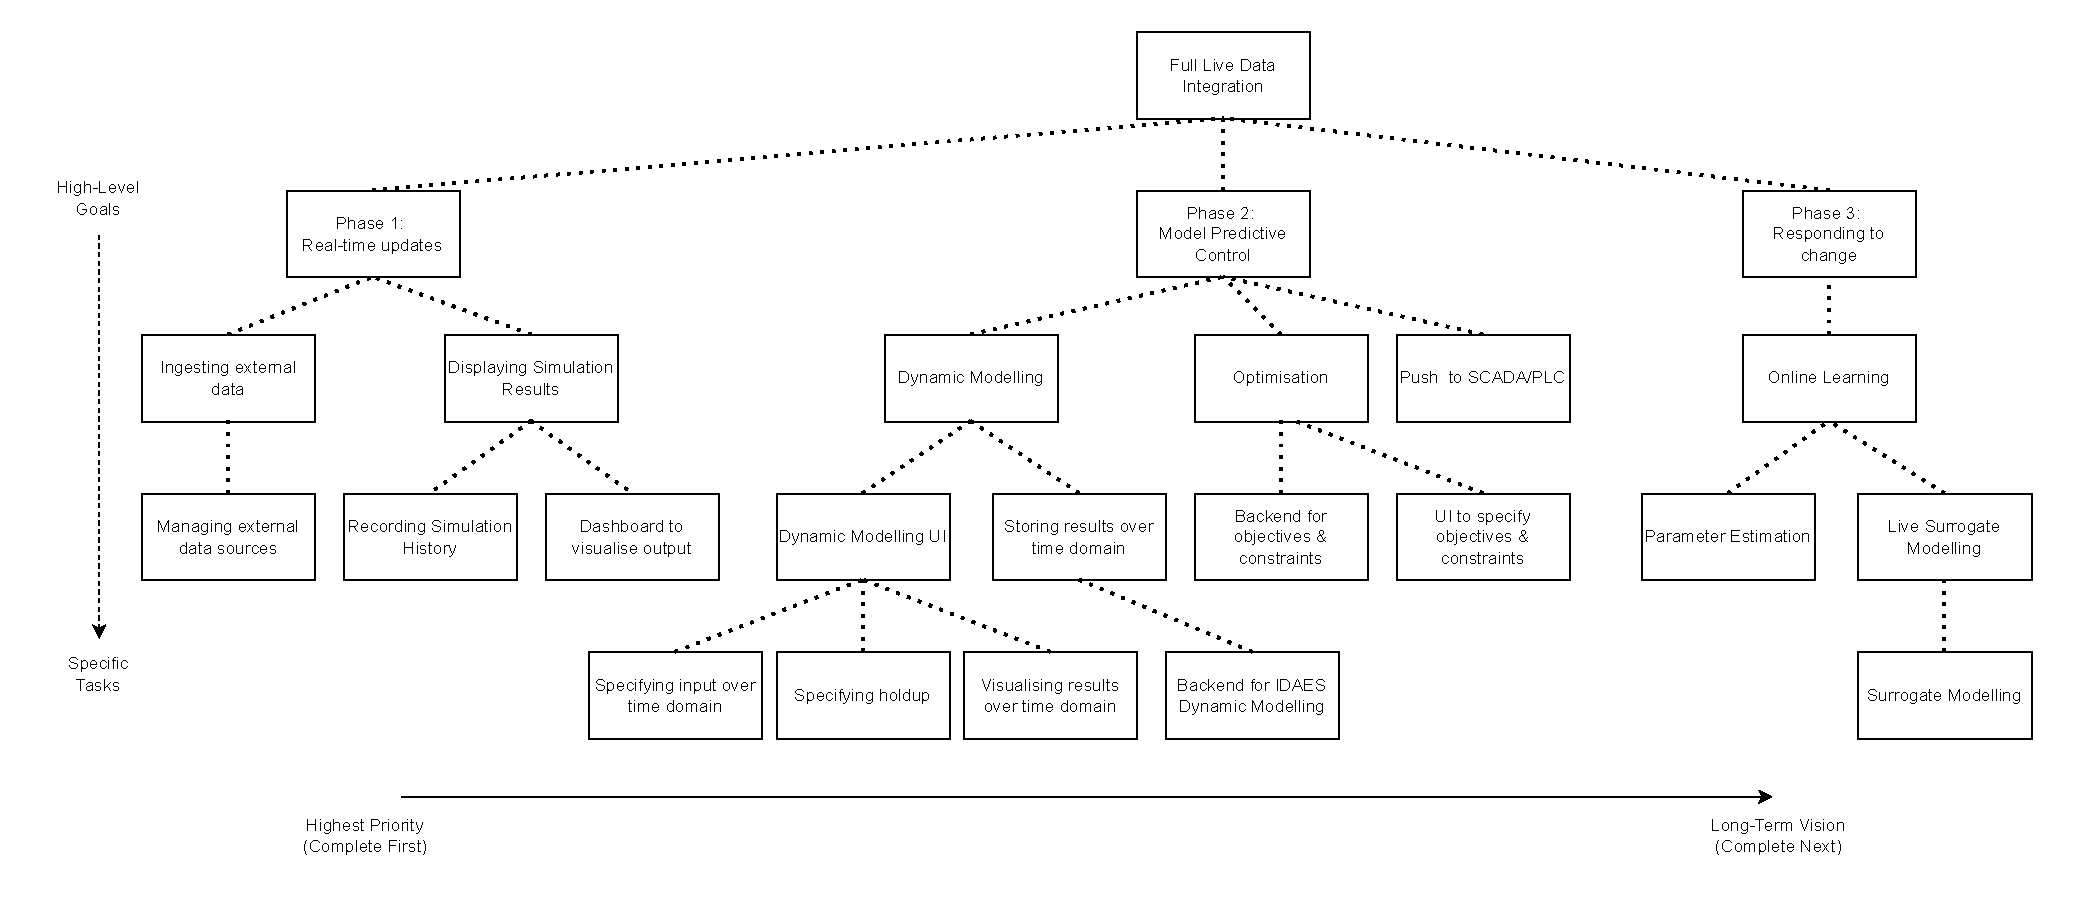
\includegraphics[width=1.5\textwidth]{roadmap.pdf}
        \caption{Roadmap of future development, broken down into tasks. This extends beyond the scope of this project, into the broader vision of the Ahuora Digital Twin Platform. Each task is a key milestone in creating an industry-ready live data processing platform.}
        \label{fig:development_flowchart}
    \end{figure}
\end{landscape}

\part{Development}
\chapter{Recording History} \label{sec:history}

Up until this point, the project has been focused on experimentation, research, and prototyping. Chapters \ref{sec:heatpumpcollection} through \ref{sec:simulationprototype} have identified key use cases, requirements, and architectures for processing live data. 
\Cref{sec:heatpumpcollection} identified that while data collection is straightforward, there are limitations to the data that can be collected. Often, custom logic for inference or sensor fusion will be required. \Cref{sec:architectureresearch} concluded that IDAES is capable of supporting dynamic modelling, surrogate modelling, optimisation, and control, but that these features mean different things in the context of live data processing compared to offline simulation. 
\Cref{sec:simulationprototype} demonstrated that the Ahuora Simulation Platform could be integrated with a real-time data processing system for steady-state modelling with relatively little effort, as long as there was a standardised API, and provided techniques to do so. However, much more complexity arises when combining all these concepts together, and when balancing the needs of the engineer's workflow with the operator's workflow.

The following chapters are focused on iteratively developing the Ahuora Simulation Platform to support live data processing, and testing these developments on the Heat Pump Dryer Model. 

\section{Purpose}

To better understand the tradeoffs of a more integrated platform, it was decided to implement a solve history system. This would allow the user to view the results of previous simulations, and compare them. It is a useful feature for the Ahuora Simulation platform as a standalone tool, but it can also be used to record the results of the real-time data processing system. A simple dashboard can be created to view past solving results, which can show how the system has changed over time. If significant advantages are found in this approach, it may be worth considering a more integrated system. If not, it can provide some insight into how to break the system apart while retaining similar functionality.


\section{Development} \label{sec:recordinghistorydevelopment}

The Ahuora Simulation platform stores all simulation results in a database after they are returned from IDAES. A table was created to store the history of previous simulations, and new entries were automatically added each time the simulation was run. Then, a user interface was created to view the results of the simulations.
% include some screenshots of the data tables, and the chart creation system.

\begin{figure}
    \centering
    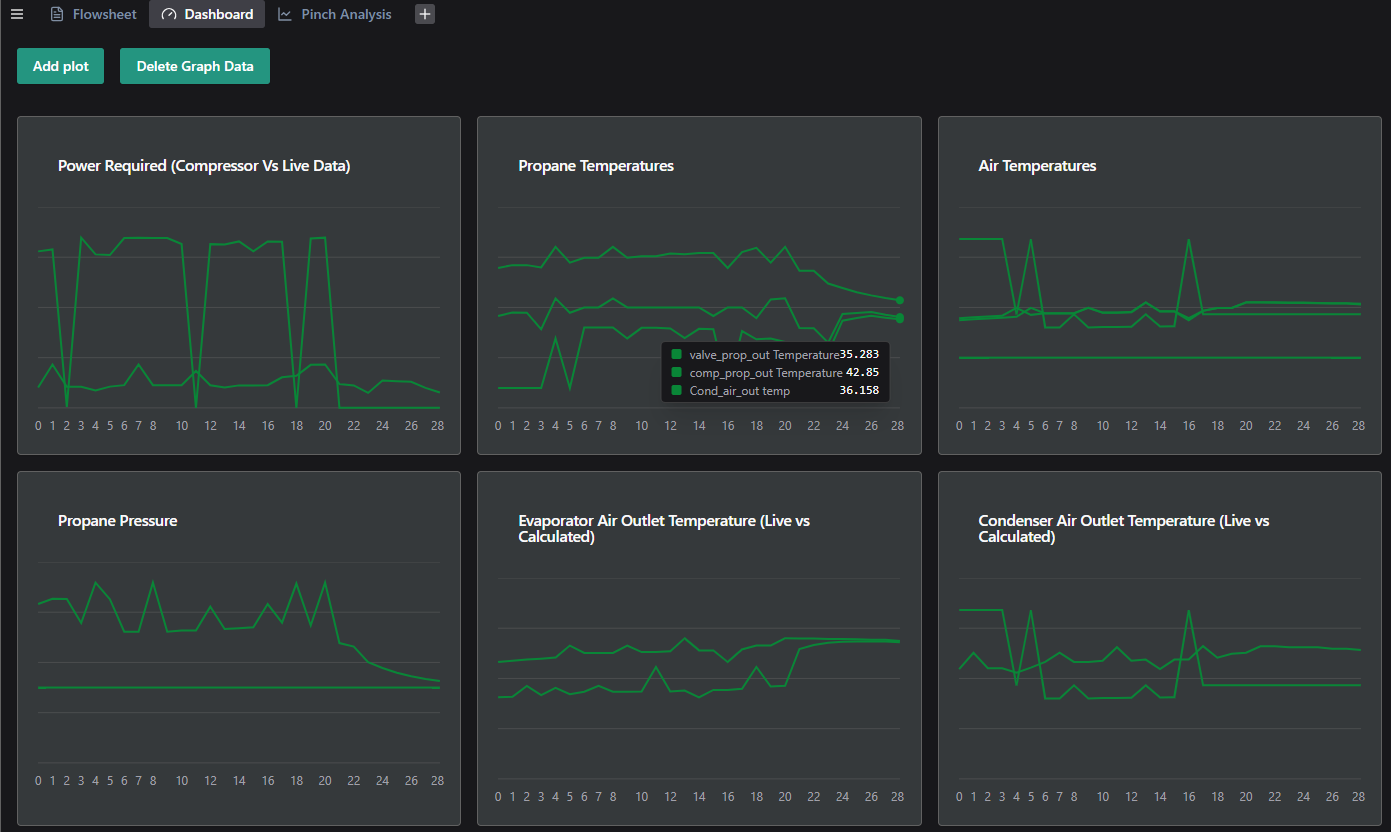
\includegraphics[width=\textwidth]{livedatadashboard.png}
    \caption{Live Data Dashboard in the Ahuora Digital Twin Platform}
    \label{fig:livedatadashboard}
\end{figure}

\Cref{fig:livedatadashboard} shows the user interface with a number of manually created graphs for the heat pump dryer. A seperate tab has been added to the Ahuora Simulation Platform to show the graphs of previous simulation results. 


\section{Testing}

The data collection scripts from \Cref{sec:heatpumpcollection} were updated to store the results in the Ahuora Simulation Platform instead of InfluxDB, using similar methods as in \Cref{sec:simulationprototype}. A heat pump was modelled in the Ahuora Simulation Platform. At this stage, the Ahuora Simulation Platform could reliably solve heat pumps with pure components, and as the heat pump dryer used propane as a refrigerant, it was a good test case. 


\begin{figure}
    \centering
    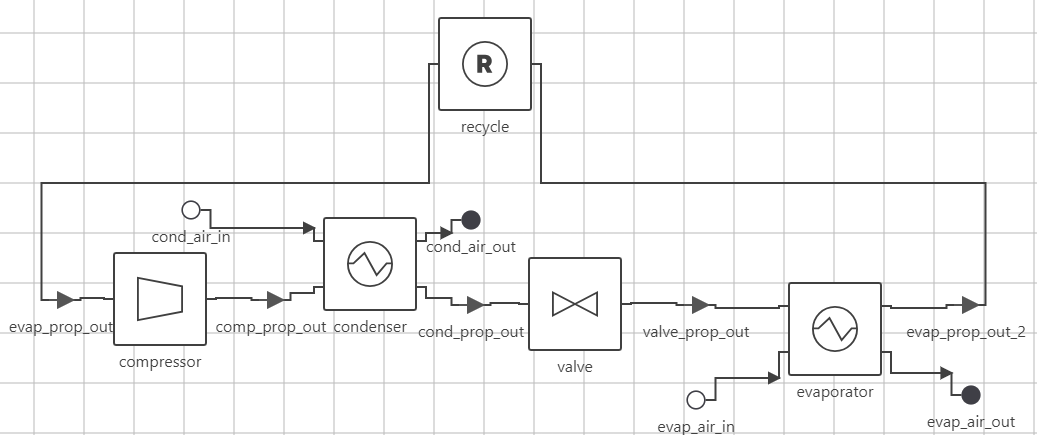
\includegraphics[width=\textwidth]{heatpumpmodel.png}
    \caption{Heat Pump Model used for live data}
    \label{fig:heatpumpmodel}
\end{figure}

\Cref{fig:heatpumpmodel} shows the heat pump model built in the Ahuora Simulation platform for this test. There are four unit operations in this model:

\begin{itemize}
    \item The compressor pressurizes the propane gas, heating it up at the same time. 
    \item The condenser cools down the propane, and the propane liquifies. The heat that leaves the propane moves into the internal drum of the dryer.
    \item The propane then moves through the valve, which reduces the pressure significantly. This causes the propane to vaporise, and the temperature further decreases to well below room temperature.
    \item Lastly, the propane moves through the evaporator, where it collects heat from the ambient surroundings, back to its original temperature.
    \item The recycle block is not a unit operation, but it specifies that the propane from the evaporator is fed back round into the inlet of the compressor. This means that the temperature, pressure, and flow rate out of the evaporator is the same as into the compressor.
\end{itemize}

The complexity arose in linking the data from the real-world sensors to the data from the simulation. In the data collection configuration the dryer was set up for, a sensor is used to read the temperature of the propane leaving the compressor, and out of the evaporator. Additionally, air temperatures are also measured, and the total power of the dryer is measured. Other properties required to calculate the flowsheet needed to be hardcoded, as shown in \Cref{tab:tempconditions}. 
The sensor readings that were measured, but not used in calculating the flowsheet are shown in \Cref{tab:liveprops}. The reason not all sensor data was used is because of two reasons: first, the air temperature readings would also require knowing the flow rate of the air and propane, which were unknown. Second, they would over-define the simulation which would make solving infeasible. 
As there were no pressure sensors, the pressure of the propane could not be measured. Thus, hand-calculations were performed to calculate what feasible pressures the propane would be at, for it to boil below room temperature and at approximately 70~\degree~C. The model performance would not always exactly reflect real-world conditions, but it would be a good enough proof of concept to see if the process worked.

The Ahuora Simulation Platform did not support specifying the outlet temperature of a compressor or valve, when these make more sensible calculation modes than outlet pressure for our avaliable live data. These were added to support this workflow.

\begin{table}[htbp]
    \centering
    \caption{Specified properties in heat pump model}
    \label{tab:tempconditions}
    \begin{tabular}{|c|c|c|}
        \hline
            \textbf{Unit Operation} & \textbf{Property} & \textbf{Source} \\
            \hline
            Compressor & Outlet Temperature & Probe Temperature Sensor \\
            Compressor & Isentropic Efficiency & Hardcoded to 100\% \\
            Condenser & Air Inlet Temperature & Hardcoded to 20 \degree C \\
            Condenser & Propane Outlet Temperature & Hardcoded to 40 \degree C \\
            Valve & Outlet Pressure & Hardcoded to 6 bar \\
            Evaporator & Air Inlet Temperature & Dryer Temperature Sensor \\
            Evaporator & Propane Outlet Temperature & Probe Temperature Sensor \\
        \hline
    \end{tabular}
\end{table}

\begin{table}[htbp]
    \centering
    \caption{Other sensor readings, not used in solving}
    \label{tab:liveprops}
    \begin{tabular}{|c|c|c|}
        \hline
            \textbf{Unit Operation} & \textbf{Property} & \textbf{Reason} \\
            \hline
            Condenser & Air Outlet Temperature & Can be calculated from propane outlet temperature \\
            Evaporator & Air Outlet Temperature & Can be calculated from propane outlet temperature \\
            Entire Dryer & Power Usage & Doesn't map cleanly to one property \\
        \hline
    \end{tabular}
\end{table}

As the Ahuora Simulation Platform could only store solving results, additional ``dummy'' unit operations were added to the flowsheet to store the other sensor readings mentioned in \Cref{tab:liveprops}.

The live data processing script was then started and run with the developed model as specified.
While the model was thermodynamically valid as it was built, and could solve correctly, it quickly started to fail to solve when being solved on the live data. 
Sometimes, IDAES would fail to initialize the models. Other times, the IPOPT solver found that either the model was infeasible, or the problem failed in restoration phase (which could be from poor scaling, inaccurate results, or it could not find a feasible starting point for solving).

It is likely there are a number of causes for this. Partially, the failed solves could be due to the hardcoded values being inaccurate, resulting in models that do not solve correctly. However, another reason is that the dryer does not exactly follow the cycle correctly when it is being started up, as initially the entire system is at room temperature. It takes some time for everything to reach steady state. 
Also, the dryer goes through a number of states - the compressor is not always running and the drum starts rotating in the other direction. During this process the simulation may not correctly model the system, potentially resulting in infeasible solutions. 
Finally, the model is trying to solve everything as a steady state - wheras in reality it takes time for changes in temperature to propagate through the entire system. 


\section{Results \& Insights}

This identified a number of problems with the current ways of handling live data.

Firstly, there needs to be a better way to handle failed solves. The only data that the flowsheet history stored was data on successful solves. When debugging solving, it would be much more useful to store successful and failed solve states. However, it may not make sense to store failed solve results in the Ahuora Simulation Platform, as the results from idaes are useless in that case. 
Perhaps an external data pipeline should do this. Additionally, the Ahuora Simulation Platform only stores properties of unit operations in the solve, making it hard to add additional data such as timestamps, or other data collected from sensors. It doesn't provide a fully-fleged data processing platform. 
In the test example, additional "dummy unit operations" disconnected from the main flowsheet were used to store the data, but this is a workaround and shouldn't be required. It also wouldn't work for other types of data, e.g if images were taken of the plant over time. From this, we can conclude that it is not appropriate for the Ahuora Digital Twin platform to form the entire knowledge base of a plant.

Secondly, the methods of specifying unit operations can vary, and the Ahuora Simulation Platform will need to support a wide number of calculation modes - in this case, an additional calculation mode (Outlet Temperature) had to be added to the compressor in order to solve the model. On discussing these results with other colleagues who are chemical engineers, they mentioned that it is common to have to calculate properties in roundabout ways. 
For example, you can calculate temperature by how much a pipe expands, or the pressure of a valve outlet from its temperature, assuming it's in the two-phase region (transitioning between liquid and gas) and is a pure fluid. The Ahuora Simulation Platform has ``Specification Blocks'' on it's roadmap of future development, which allow specifying arbitrary relationships between variables. This may help with these sorts of scenarios - or it can be treated as a preprocessing step before feeding the calculated values into the Ahuora Simulation Platform.

There was a lot of data that couldn't be used in the Ahuora Simulation Platform. This could have been used if the Ahuora Simulation Platform allowed more flexible model specification: the inlet and outlet air temperatures could have been used to calculate the heat capacity of the air streams, or efficiency of the heat exchangers.
Alternatively, overspecified data could be used for sensor fusion as explained in the Literature Review (Appendix \ref{sec:litreview}), using Bayesian statistics to calculate what the most probable true values are and the uncertainty associated with them. 
However, this would significantly increase the complexity of the model; an alternative is just to compare the simulation output to the live data, and flag any significant variations as a potential problem. 
Sensor fusion would likely require bayesian methods to be implemented into the Ahuora Simulation Platforms, comparing variances could be done as a postprocessing step in a seperate software.

%TODO: Link all the use cases together in the proposed system architecture section.
This all provides cause for reflection on the use cases identified in \Cref{sec:researchconclusions}, \Cref{tab:requirements}. While both the engineer's use case and the operator's use cases are still valid, there was an assumption that the person setting up the digital twin would be able to easily port an engineer's model (e.g, from the design of a plant) into a digital twin that processes live data; that it would be just a matter of linking the model up with a live data source. From this test, it is clear that finding the correct parameters to define a model, and finding a way to link sensor readings up with simulation parameters, is a non-trivial task: it is not as straightforward as a one-to-one mapping. Thus, two other use cases should be considered. A ``Data Engineer'' may be a Software Engineer responsible for aggregating data from different sensors (and simulation results) into a single SCADA system or Industrial IoT system. A ``Process Engineer'', for want of a better term, may be a Chemical Engineer who is responsible for linking existing simulation models with the IoT data, using their domain specific knowledge to convert the IoT readings from sensor outputs into valid parameters for a simulation model, using sensor fusion or other techniques. These need to be considered alongside the requirements of a chemical engineer only focused on design, and a operator only focused on control.

\begin{table}[ht]
    \centering
    \caption{Comparison of a Data Engineer's and a Process Engineer's workflow}
    \begin{tabular}{|c|p{0.35\textwidth}|p{0.4\textwidth}|}
        \hline
        \textbf{Requirement} & \textbf{Data Engineer} & \textbf{Process Engineer} \\
        \hline
        Use Case & Integrating simulation results into company knowledge base & Convert sensor readings into model parameters \\
        \hline
        Skillset & Software, Networking, Data Storage, and Data Processing  & Chemical Modelling, Data Processing \\
        \hline
        Modelling & Doesn't do chemical modelling & Extends the model with sensor fusion \& preprocessing techniques\\
        \hline
        Requirements & Good API to interface with the platform & Easy to use tools and techniques for sensor fusion \\
        \hline
        Historical Data & Needs to store historical data & Needs to test models on historical data \\
        \hline
    \end{tabular}
    \label{tab:morerequirements}
\end{table}


\Cref{tab:morerequirements} summarises the requirements of each of these new use cases. The data engineer is most concerned about integration with existing systems. This would be best serviced by ensuring the data processing platform in Ahuora has simple, clear APIs to ingest data and extract data after solve. The Process Engineer wants easy access to all the sensor data in the factory, and sufficient tooling to be able to convert the sensor data into model parameters. This could be achieved by adding additional model properties to the Ahuora Simulation Platform, but more complex cases may require additional pre/postprocessing outside of the IDAES solver. Exactly what this could entail is highly implementation-specific.

\section{Discussion}

% TODO: Consider how this relates to the previous chapter and how it sets things up to the next chapter, adjust them so they're consistent.

In the previous chapter, \Cref{sec:prototypeinsights} discussed the tradeoffs between doing everything in the Ahuora Platform, and doing as much as possible in an external system. The insights gained in this chapter suggest that the Ahuora Simulation platform alone is insufficient, and that linking with external systems would be required to store results in line with other company data. This also enables more advanced processing techniques to be implemented through custom logic outside of the Ahuora Platform. However, specific techniques that involve extending the mathematical model of the system would be best done in the Ahuora Simulation Platform. A seperate suite of tools to handle a data processing pipeline would best support this, though a full implementation would be a significant undertaking that is beyond the scope of this project. 

Additionally, a Process Engineer, who is not as skilled at software engineering or programming, would be best served by having some data preprocessing tools built into the platform. As an integrated solution, they could test their models on historical data, using platform tools for data processing. A Data Engineer could then be responsible for providing the required live data to the platform, and storing simulation results, without having to deal with the intracacies of the model itself.




\section{Improving Solving Reliability} \label{sec:solvingreliability}

% Talk about why initialisation could be a failing point, how to fix that (e.g remove the recycle, or save initialisation states)
As the solving for the heat pump dryer was not always successful, some additional time was spent to improve the reliability of solving.
This helped to identify relevant preprocessing steps to implement in the platform.
There are a couple of reasons why the solving of the flowsheet was not always successful in the previous section. 

The first reason is that the heat exchangers could be failing to initialise. They are the most complex unit operation, and require appropriate fluid volumes, heat deltas, flow transfer areas, and heat transfer coefficients to be set. If these are not set correctly, the heat exchanger may not initialise. 

As in this model we did not have flow rates for the air inlets, approximate values were being used. Thus including heat exchangers in the model did not provide any more accuracy, and only added complexity. The model was updated with heaters and coolers instead of heat exchangers, which can be solved much more reliably.

The second reason why the model may not have been solving is that the recycle loop was not being initialised correctly. The recycle stream was being set to the same value as the outlet stream, but this creates a continuous loop that the solver may not be able to solve at a steady state. For the next test, the recycle was removed, and the tear guess values were used as the initial conditions. 

% TODO: picture of the data (look it's not so sparodic anymore)

When both of these changes were made, the model was able to solve reliably. The results of the simulation were much more consistent, and better reflected the expected behaviour of the heat pump dryer.


While implementing this, another issue was discovered. Because stream properties were being used to store additional live data that was not part of the simulation, sometimes the live data was invalid as a stream condition. This was done so the part of the platform that recorded solve history could be used to display all live data results, not just the simulation results. However, this was not a good solution, as it made the simulation less reliable. This means that either the solve history feature should be updated to handle storing additional metadata, or the live data should be stored in a different way.


% Todo: figure out a bit more of a structure for this

% Maybe mention scaling?

% is there any other preprocessing steps we could do? Should we add specification blocks?

% what does this prove about the architecture?


%
\chapter{Improving Solving Reliability} \label{sec:solvingreliability}

% Talk about why initialisation could be a failing point, how to fix that (e.g remove the recycle, or save initialisation states)

There are a couple of reasons why the solving of the flowsheet was not always successful in the previous section. 

The first reason is that the heat exchangers could be failing to initialise. They are the most complex unit operation, and require appropriate fluid volumes, heat deltas, flow transfer areas, and heat transfer coefficients to be set. If these are not set correctly, the heat exchanger may not initialise. 

As in this model we did not have flow rates for the air inlets, approximate values were being used. Thus including heat exchangers in the model did not provide any more accuracy, and only added complexity. The model was updated with heaters and coolers instead of heat exchangers, which can be solved much more reliably.

The second reason why the model may not have been solving is that the recycle loop was not being initialised correctly. The recycle stream was being set to the same value as the outlet stream, but this creates a continuous loop that the solver may not be able to solve at a steady state. For the next test, the recycle was removed, and the tear guess values were used as the initial conditions. 

% TODO: picture of the data (look it's not so sparodic anymore)

When both of these changes were made, the model was able to solve reliably. The results of the simulation were much more consistent, and better reflected the expected behaviour of the heat pump dryer.


While implementing this, another issue was discovered. Because stream properties were being used to store additional live data that was not part of the simulation, sometimes the live data was invalid as a stream condition. This was done so the part of the platform that recorded solve history could be used to display all live data results, not just the simulation results. However, this was not a good solution, as it made the simulation less reliable. This means that either the solve history feature should be updated to handle storing additional metadata, or the live data should be stored in a different way.


% Todo: figure out a bit more of a structure for this

% Maybe mention scaling?

% is there any other preprocessing steps we could do? Should we add specification blocks?

% what does this prove about the architecture?


\chapter{Data Preprocessing} \label{sec:datapreprocessing}

% It's required because process engineers get raw sensor data and need to aggregate it etc for the model.
% However, they also need to work from historical data to test the model, and to understand the system.

% This is also part of multi-steady-state and pretty helpful anyway for chemical engineers too.


% IT was implemented using XYZ, because XYZ so that ABC
% also, we decided that ... because ... so that ...




\section{Motivation}

\section{Method}

\chapter{Proposed System Architecture}
% Digital Twin Software needs to suit the use cases of Network Administrators, Chemical Engineers, Process Engineers, and Operators to be useful in industry.
% Steady-State, Dynamic, and Surrogate modelling are all required to support the different use cases.
% A Digital Twin platform needs to integrate with existing SCADA systems and data processing tools to be useful in industry.

% Simulation results need to be avalible within the platform, but this should not replace the company's existing knowledge base/data lake/logging.
% There is no need for Ahuora to develop a new data processing platform, as SCADA systems or things such as kafka/mqtt do this fine.
% It should be easy to switch between design and operation modes, assuming the network administrator has set up the external data processing platform/sources.
% The Ahuora Digital Twin Platform needs to be designed to support these requirements.


\chapter{Conclusions}

% This chapter summarises your project, including a concise and significant summary of the R&D project findings, and contributions. 

% Present the outcome, and the arguments.
% Link back to research questions

%\section{Objectives \& Outcomes}


%\section{Research}

The research conducted in this project has identified where the key areas of work are in developing a Digital Twin Platform for Ahuora. 
This has resulted in a framework being proposed for the system, wherein the Digital Twin Platform is built on top of a data processing pipeline and a simulation platform. 
It has been tested via prototyping to show that it is appropriate for those who are involved in both design and operation of the factory, from a data or chemical engineering perspective.

%\section{Development}

This has been implemented in the Ahuora Digital Twin Platform for steady-state modelling. 
The ability to store solve history was added to visualise the results of simulations, and functionality to preprocess data was added to make it possible to convert input data to the format required in chemical modelling. 

As a test case, a model of a heat pump dryer was created and the platform was used to simulate the dryer's performance. 
This showed that the platform is capable of simulating a factory's performance, and identified some edge cases where care must be taken to specify the model in a way that it can be reliabily solved.

This work addressed some of the main challenges in implementing digital twins in the industry, namely, the complexity and cost of building a Digital Twin system from scratch. Through the continued development of Digital Twin Platforms as specified in this report, Project Ahuora's goal to decarbonise the process heat sector will be fully realised.

%\section{Future Work}
% Strengths, limitations, impacts, what could have been better, etc


\section{Future work}
% TODO: Update this section from the interlude
Future work could focus on adding support for dynamic models, hybrid modelling, and optimisation to the Ahuora Platform. Then the live data processing system could be developed to support these features. 
This would increase the usefulness of the platform for factory operation and control. 


The research conducted so far has provided the context required to build a high-level roadmap of future development. This is provided in Appendix \ref{app:roadmap}.



Further work should also be performed on the feasibility of creating a standalone `Deployment' version of the Ahuora Platform, specifically focused on control and optimisation. The research presented in this report implies that such a product would better fit the constraints of a real factory, in cases where cloud platforms may not be appropriate.

%\section{Impact Statement}


% evaluates the broader impact of the project outcome, either quantitatively or qualitatively (e.g., social, economic, environmental, health, safety, legal, ethical, and/or cultural issues)
%\section{Impact}





\bibliographystyle{unsrt}
\bibliography{refs} % Entries are in the refs.bib file

\begin{appendices}

\chapter{Heat Pump Dryer Model} \label{app:heatpumpmodel}


\chapter{Project Proposal} \label{sec:proposal}
    % The project proposal is included as an appendix on the following page.


    % 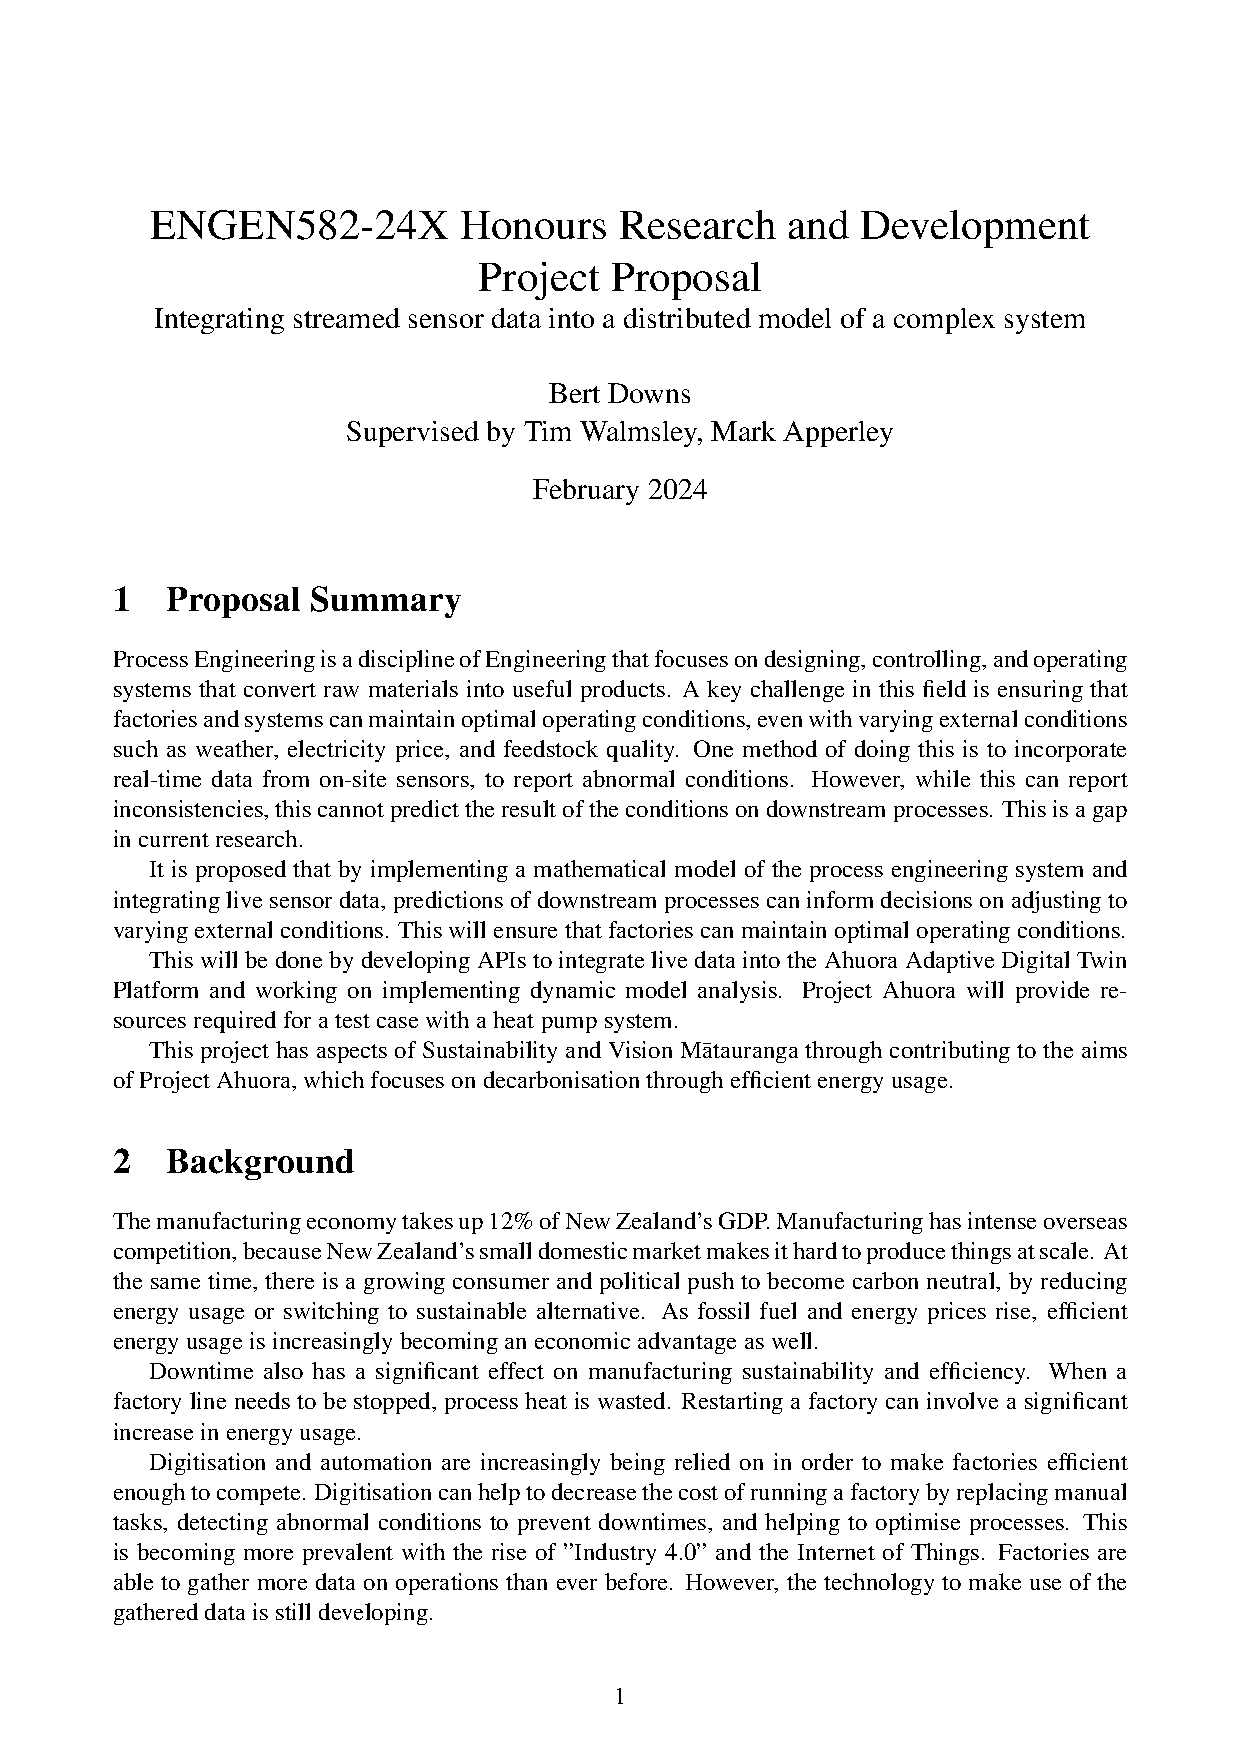
\includepdf[pages=1-4]{proposal.pdf}

    % \begin{landscape}
    %     \includepdf[pages=5,angle=90]{proposal.pdf}
    % \end{landscape}

\chapter{Literature Review} \label{sec:litreview}
    % The literature review is included as an appendix on the following page.

    % 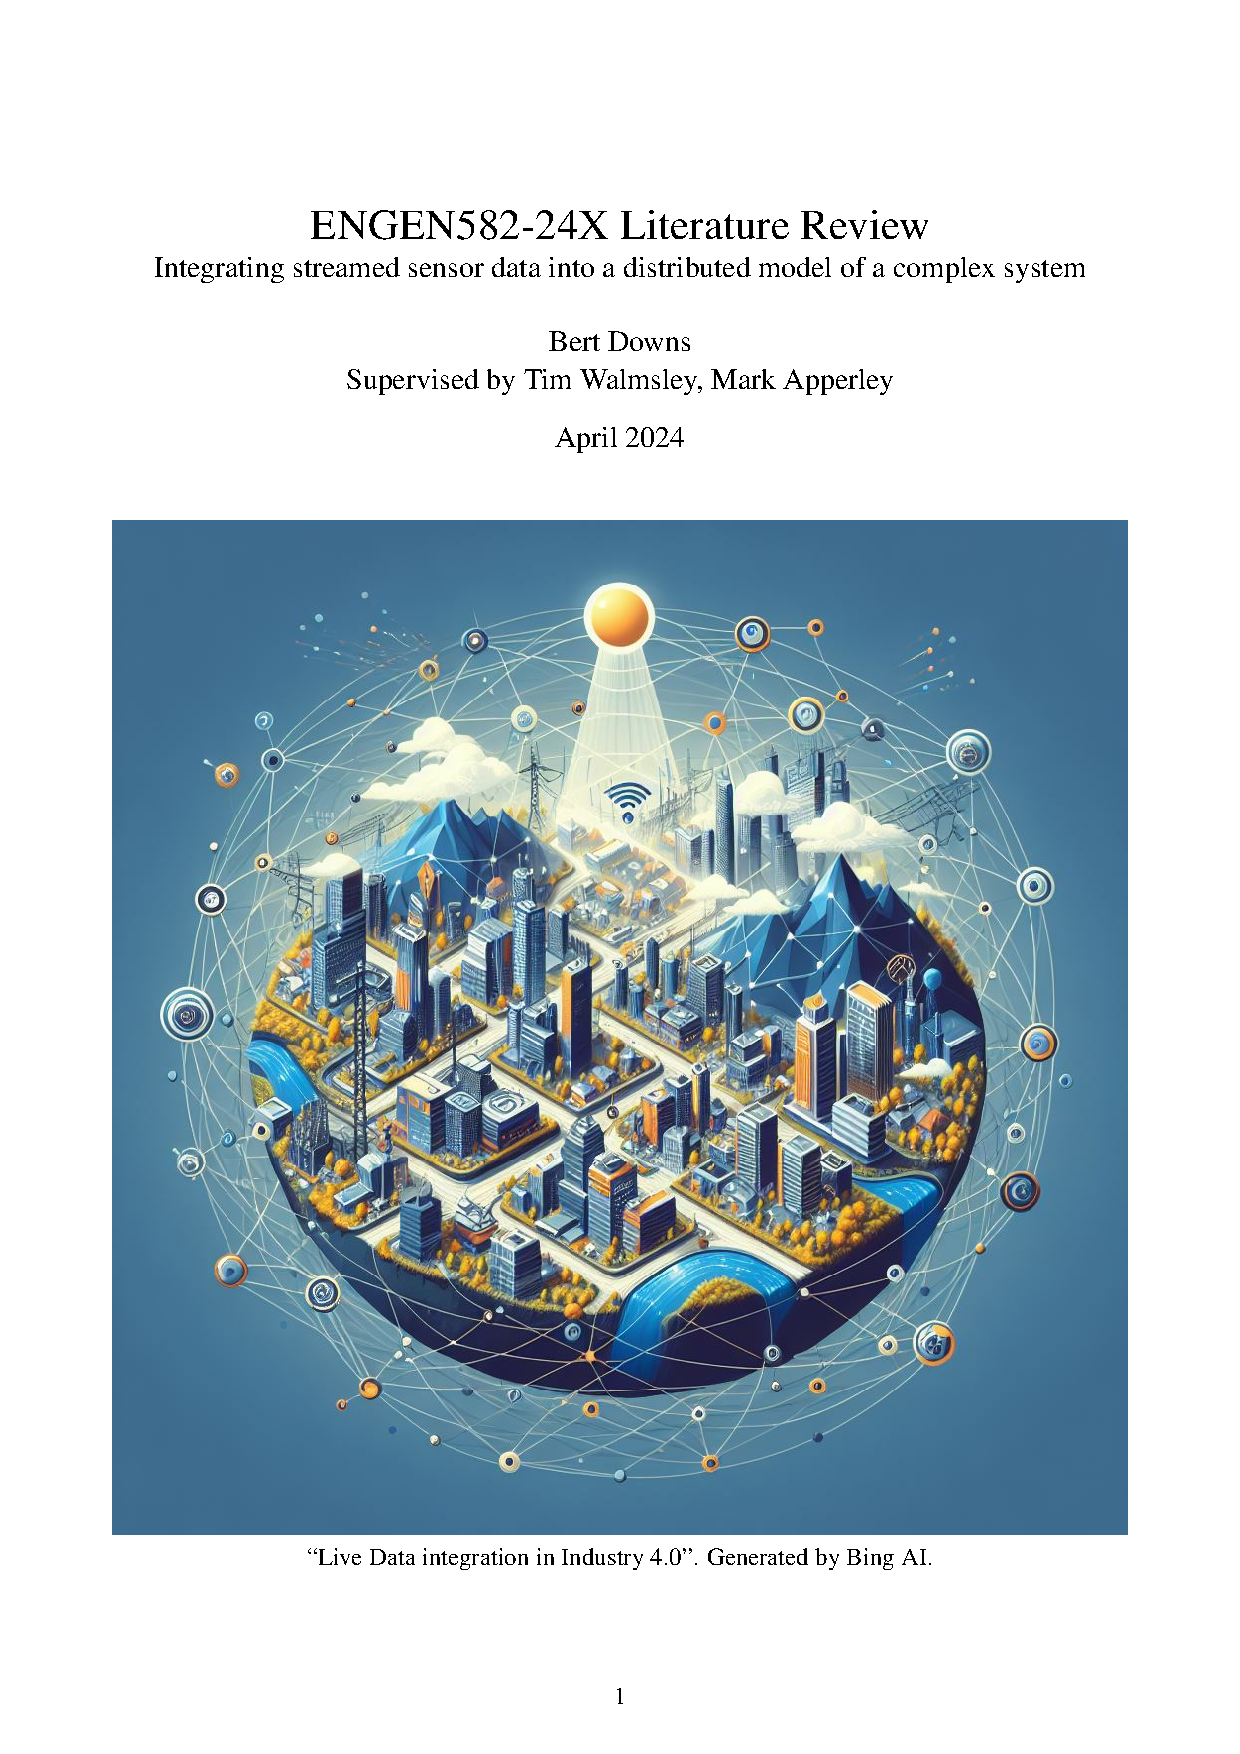
\includepdf[pages=-]{literature_review.pdf}

\end{appendices}
\end{document}


